\chapter{Arhitektura i dizajn sustava}
		
        Rehub predstavlja sofisticirano arhitektonsko rješenje koje integrira PostgreSQL bazu podataka, Spring Boot za backend logiku, React za korisničko sučelje, te Tailwind CSS za moderno i responzivno oblikovanje. Sustav je implementiran na cloud platformama Render za backend i bazu te Netlify za frontend, koristeći njihove usluge za brz, skalabilan i pouzdan deploying.\\

            \begin{packed_item}
                \large \item Baza podataka: PostgreSQL \normalsize \\
                    PostgreSQL, snažan sustav za upravljanje relacijskim bazama podataka, predstavlja ključnu komponentu u arhitekturi ove web aplikacije. Struktura baze podataka temeljito je dizajnirana kako bi zadovoljila specifične zahtjeve aplikacije. Kroz pažljivu integraciju s PostgreSQL-om, aplikacija ostvaruje brz i učinkovit pristup podacima, čime se osigurava optimalna performansa. Ova konfiguracija baze podataka predstavlja ključnu komponentu cjelokupnog arhitektonskog rješenja, pružajući čvrstu temeljnu strukturu za rad backend sustava. \\
                \large \item Backend: Spring Boot \normalsize \\
                    Spring Boot, kao Java-based framework, pruža snažan temelj za razvoj backend logike. Ova web aplikacija koristi Spring Boot za stvaranje RESTful API-ja koji komunicira s PostgreSQL bazom podataka. Ovo rješenje omogućuje efikasno upravljanje podacima i pruža mogućnost proširivosti sustava kroz modularnost i lakoću integracije. \\
                \large \item Frontend: React \normalsize \\
                    React, centralna JavaScript biblioteka, određuje arhitekturu frontend dijela ove aplikacije. Modularne React komponente omogućuju čist i jednostavan kod, prilagodljiv specifičnim zahtjevima sučelja. Ovaj pristup omogućuje stvaranje brzog, dinamičkog korisničkog sučelja koje se lako održava. Kroz React, osigurava se fluidna navigacija kroz aplikaciju, pridonoseći ukupnom intuitivnom korisničkom iskustvu. \\
                \large \item Frontend Integracija: Tailwind CSS, Axios, React-Router-Dom, reCAPTCHA \normalsize \\
                    Frontend aplikacije unaprijeđen je integracijom Tailwind CSS za brzo oblikovanje sučelja, Axios za efikasnu komunikaciju s backendom, React-Router-Dom za fluidnu navigaciju te reCAPTCHA sustava radi dodatne sigurnosti. Tailwind CSS pridonosi estetskom izgledu, Axios omogućuje dinamičku interakciju s backendom, React-Router-Dom olakšava upravljanje rutama, dok reCAPTCHA sprječava zlonamjerne aktivnosti. Kroz ovu integraciju postiže se uravnoteženo frontend rješenje koje kombinira funkcionalnost, estetiku i sigurnost korisničkog iskustva. \\
                \large \item Deployment: Render za backend i Netlify za frontend \normalsize \\
                    Backend i baza podataka su postavljeni na Render platformu za optimalno upravljanje resursima. Render osigurava automatsko skaliranje i brzu dostupnost aplikacije koristeći njihove cloud usluge. Na renderu je također podešeno kontinuirano postavljanje koje omogućuje automatsko ažuriranje softvera. Frontend je zasebno postavljen na Netlify platformi, koja pruža brzo i globalno dostupno CDN (Content Delivery Network). \\
            \end{packed_item}

            Rehub predstavlja integrirano arhitektonsko rješenje koje kombinira najbolje prakse u razvoju aplikacija, pružajući stabilnost, skalabilnost i visoku razinu korisničkog iskustva. Korištenje navedenih tehnologija i servisa osigurava da aplikacija bude spremna za izazove suvremenog web razvoja.
           

                
            
                \begin{figure}[H]
			         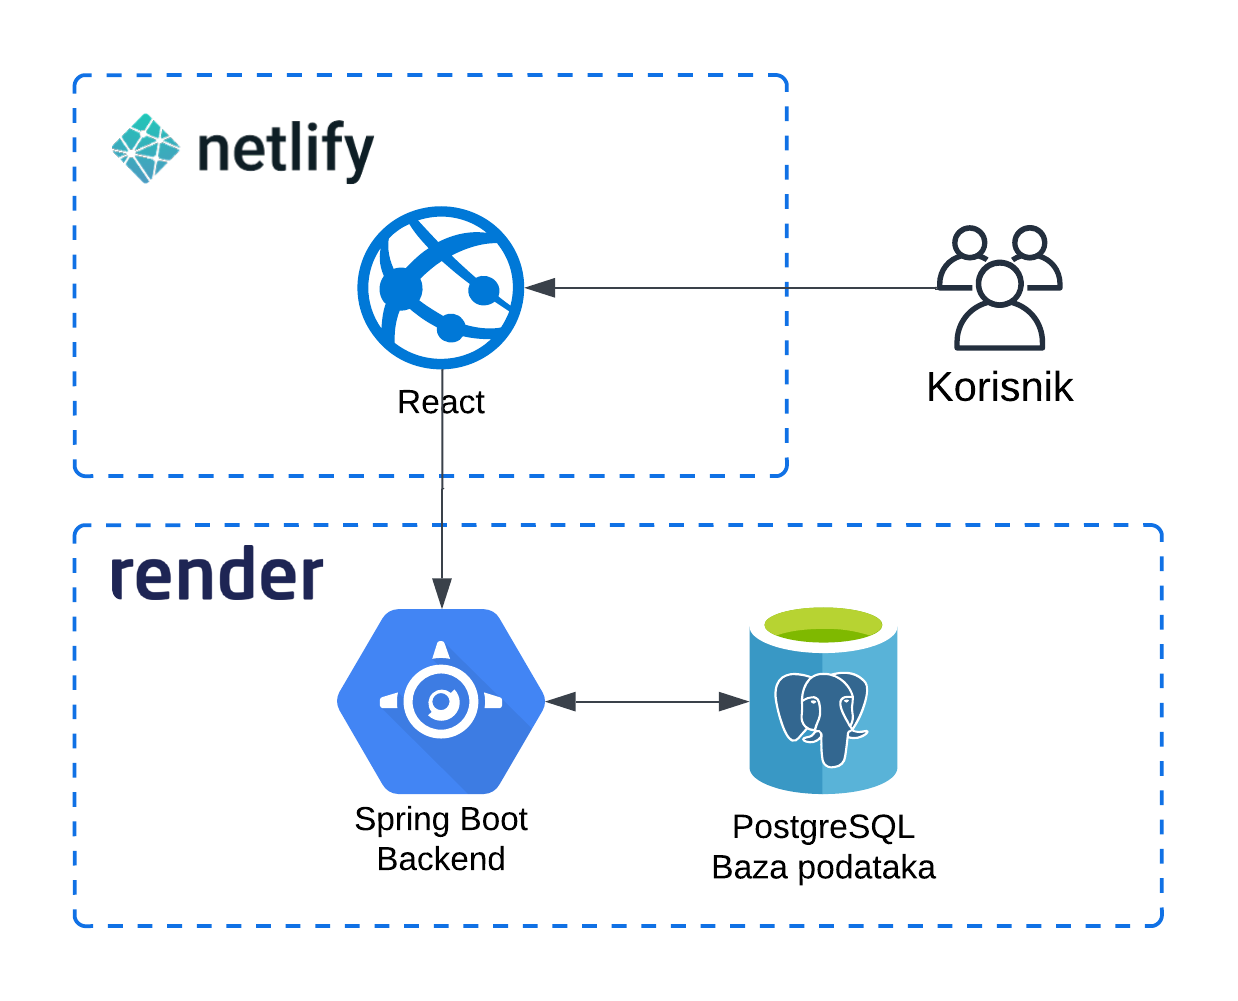
\includegraphics[scale=0.25]{dijagrami/architecture_diagram.png}
			         \centering
			         \caption{Dijagram arhitekture}
			         \label{fig:architecture_diagram}
		        \end{figure}

		\section{Baza podataka}
			
		U bazi su stvorene relacije koje olakšavaju jednostavno rukovanje podacima, uključujući dodavanje, brisanje, izmjenu i dohvaćanje podataka. Svi entiteti i relacije su organizirani prema trećoj normalnoj formi kako bi se izbjegla redundancija podataka. Za bolje vizualiziranje strukture baze podataka, napravljen je relacijski dijagram koji je prikazan u nastavku. \\
        \\
        Baza podataka se sastoji od tablica (relacija) koje su definirane svojim imenom i skupom
atributa. Baza podataka ove aplikacije sastoji se od sljedećih entiteta:

            \begin{packed_item}
                \item rehub\_user
                \item employee
                \item user\_role
                \item role
                \item patient
                \item therapy
                \item therapy\_result
                \item doctor
                \item appointment
                \item room
                \item equipment
                \item faq
                \item personal\_data
                \item flyway\_history\_schema
            \end{packed_item}

		
			\subsection{Opis tablica}
			
			 Prva ćelija svake tablice označava njeno ime. U prvom stupcu navedeni su atributi tog entiteta, u drugom stupcu naveden je tip varijable, a u trećem opis svakog pojedinog atributa. Svjetlozelenom bojom označeni su primarni ključevi. Svjetlo plavom označeni su strani ključevi. \\	

				
				\begin{longtblr}[
					label=none,
					entry=none
					]{
						width = \textwidth,
						colspec={|X[6,l]|X[6, l]|X[20, l]|}, 
						rowhead = 1,
					} %definicija širine tablice, širine stupaca, poravnanje i broja redaka naslova tablice
					\hline \SetCell[c=3]{c}{\textbf{rehub\_user}}	 \\ \hline[3pt]
					\SetCell{LightGreen}ID & BIGSERIAL	&  	JEDINSTVENI IDENTIFIKATOR KORISNIKA  	\\ \hline
					USERNAME	& VARCHAR &   KORISNIČKO IME S KOJIM SE KORISNIK PRIJAVLJUJE	\\ \hline 
					PASSWORD & VARCHAR &  LOZINKA S KOJOM SE KORISNIK PRIJAVLJUJE \\ \hline 
				\end{longtblr}
                Entitet označava korisnika aplikacije te sadrži atribute: id, username, password.\\

                \begin{longtblr}[
					label=none,
					entry=none
					]{
						width = \textwidth,
						colspec={|X[6,l]|X[6, l]|X[20, l]|}, 
						rowhead = 1,
					} %definicija širine tablice, širine stupaca, poravnanje i broja redaka naslova tablice
					\hline \SetCell[c=3]{c}{\textbf{employee}}	 \\ \hline[3pt]
					\SetCell{LightGreen}ID & BIGSERIAL	&  	JEDINSTVENI IDENTIFIKATOR ZAPOSLENIKA  	\\ \hline
					FIRST\_NAME	& VARCHAR &   IME ZAPOSLENIKA	\\ \hline 
					LAST\_NAME & VARCHAR &  PREZIME ZAPOSLENIKA \\ \hline 
                    PHONE\_NUMBER & VARCHAR &  BROJ MOBITELA ZAPOSLENIKA \\ \hline
                    PROFESSION & VARCHAR &  STRUKA ZAPOSLENIKA \\ \hline
                    DATE\_OF\_BIRTH & DATE &  DATUM ROĐENJA ZAPOSLENIKA \\ \hline
                    GENDER & VARCHAR &  SPOL ZAPOSLENIKA \\ \hline
                    CREATED\_AT & TIMESTAMP &  TRENUTAK KREIRANJA \\ \hline
                    LAST\_MODIFIED\_AT & TIMESTAMP &  TRENUTAK ZADNJE PROMJENE \\ \hline
                    \SetCell{LightBlue} USER\_ID & VARCHAR &  JEDINSTVENI IDENTIFIKATOR KORISNIKA \\ \hline
				\end{longtblr}
                Entitet označava osobe zaposlene u klinici. Atributi ovoga entiteta su: id, first\_name, last\_name, phone\_number, profession, date\_of\_birth, gender, created\_at, last\_modified\_at, user\_id.\\

                \begin{longtblr}[
					label=none,
					entry=none
					]{
						width = \textwidth,
						colspec={|X[6,l]|X[6, l]|X[20, l]|}, 
						rowhead = 1,
					} %definicija širine tablice, širine stupaca, poravnanje i broja redaka naslova tablice
					\hline \SetCell[c=3]{c}{\textbf{user\_role}}	 \\ \hline[3pt]
					\SetCell{LightBlue} USER\_ID & BIGSERIAL	&  	JEDINSTVENI IDENTIFIKATOR KORISNIKA  	\\ \hline
					\SetCell{LightBlue} ROLE\_ID	& BIGSERIAL &   JEDINSTVENI IDENTIFIKATOR VRSTE KORISNIKA	\\ \hline 
				\end{longtblr}
                Entitet označava vrstu korisnika aplikacije, a njegovi atributi su: user\_id, role\_id.\\

                \begin{longtblr}[
					label=none,
					entry=none
					]{
						width = \textwidth,
						colspec={|X[6,l]|X[6, l]|X[20, l]|}, 
						rowhead = 1,
					} %definicija širine tablice, širine stupaca, poravnanje i broja redaka naslova tablice
					\hline \SetCell[c=3]{c}{\textbf{role}}	 \\ \hline[3pt]
					\SetCell{LightGreen} ID & BIGSERIAL	&  	JEDINSTVENI IDENTIFIKATOR ULOGE  	\\ \hline
					NAME	& VARCHAR &   IME ULOGE	\\ \hline 
				\end{longtblr}
                Entitet označava ulogu i sastoji se od atributa: id, name.\\

                \begin{longtblr}[
					label=none,
					entry=none
					]{
						width = \textwidth,
						colspec={|X[6,l]|X[6, l]|X[20, l]|}, 
						rowhead = 1,
					} %definicija širine tablice, širine stupaca, poravnanje i broja redaka naslova tablice
					\hline \SetCell[c=3]{c}{\textbf{patient}}	 \\ \hline[3pt]
					\SetCell{LightGreen} ID & BIGSERIAL	&  	JEDINSTVENI IDENTIFIKATOR PACIJENTA  	\\ \hline
					FIRST\_NAME	& VARCHAR &   IME PACIJENTA	\\ \hline 
                    LAST\_NAME	& VARCHAR &   PREZIME PACIJENTA	\\ \hline
                    GENDER	& VARCHAR &   SPOL PACIJENTA	\\ \hline
                    PHONE\_NUMBER	& VARCHAR &   BROJ MOBITELA PACIJENTA	\\ \hline
                    DATE\_OF\_BIRTH	& DATE &   DATUM ROĐENJA PACIJENTA	\\ \hline
                    CREATED\_AT	& TIMESTAMP &   TRENUTAK KREIRANJA	\\ \hline
                    LAST\_MODIFIED\_AT	& TIMESTAMP &   TRENUTAK ZADNJE PROMJENE	\\ \hline
                    \SetCell{LightBlue} USER\_ID	& BIGSERIAL &   JEDINSTVENI IDENTIFIKATOR KORISNIKA	\\ \hline
				\end{longtblr}
                Entitet predstavlja pacijenta koji je korisnik aplikacije. Atributi su: id, first\_name, last\_name, gender, phone\_number, date\_of\_birth, created\_at, last\_modified\_at, user\_id.\\

                \begin{longtblr}[
					label=none,
					entry=none
					]{
						width = \textwidth,
						colspec={|X[6,l]|X[6, l]|X[20, l]|}, 
						rowhead = 1,
					} %definicija širine tablice, širine stupaca, poravnanje i broja redaka naslova tablice
					\hline \SetCell[c=3]{c}{\textbf{therapy}}	 \\ \hline[3pt]
					\SetCell{LightGreen} ID & BIGSERIAL	&  	JEDINSTVENI IDENTIFIKATOR TERAPIJE  	\\ \hline
					TYPE	& VARCHAR &   VRSTA TERAPIJE	\\ \hline 
                    REQUEST	& VARCHAR &   ZAHTJEV ZA TERAPIJOM	\\ \hline
                    STATUS	& VARCHAR &   STATUS TERAPIJE	\\ \hline
                    REF\_ID	& BIGSERIAL &   JEDINSTVENI IDENTIFIKATOR	\\ \hline
                    CREATED\_AT	& TIMESTAMP &   TRENUTAK KREIRANJA	\\ \hline
                    LAST\_MODIFIED\_AT	& TIMESTAMP &   TRENUTAK ZADNJE PROMJENE	\\ \hline
                    \SetCell{LightBlue} PATIENT\_ID	& BIGSERIAL &   JEDINSTVENI IDENTIFIKATOR PACIJENTA	\\ \hline
                    \SetCell{LightBlue} ROOM\_ID	& BIGSERIAL &   JEDINSTVENI IDENTIFIKATOR SOBE	\\ \hline
                    \SetCell{LightBlue} DOCTOR\_ID	& BIGSERIAL &   JEDINSTVENI IDENTIFIKATOR DOKTORA	\\ \hline
                    \SetCell{LightBlue} APPOINTMENT\_ID	& BIGSERIAL &   JEDINSTVENI IDENTIFIKATOR TERMINA	\\ \hline
                    \SetCell{LightBlue} THERAPY\_RESULT\_ID	& BIGSERIAL &   JEDINSTVENI IDENTIFIKATOR REZULTATA TERAPIJE	\\ \hline
				\end{longtblr}
                Entitet opisuje terapiju dodijeljenu pacijentu. Njeni atributi su: id, type, request, status, ref\_id, created\_at, last\_modified\_at, patient\_id, room\_id, doctor\_id, appointment\_id, therapy\_result\_id.\\

                \begin{longtblr}[
					label=none,
					entry=none
					]{
						width = \textwidth,
						colspec={|X[6,l]|X[6, l]|X[20, l]|}, 
						rowhead = 1,
					} %definicija širine tablice, širine stupaca, poravnanje i broja redaka naslova tablice
					\hline \SetCell[c=3]{c}{\textbf{doctor}}	 \\ \hline[3pt]
					\SetCell{LightGreen}ID & BIGSERIAL	&  	JEDINSTVENI IDENTIFIKATOR DOKTORA  	\\ \hline
					FIRST\_NAME	& VARCHAR &   IME DOKTORA	\\ \hline 
					LAST\_NAME & VARCHAR &  PREZIME DOKTORA \\ \hline 
                    PIN & VARCHAR &  PIN DOKTORA \\ \hline 
                    PHONE\_NUMBER & VARCHAR &  BROJ MOBITELA DOKTORA \\ \hline 
                    SPECIALITY & VARCHAR &  DOKTOROVA SPECIJALIZACIJA \\ \hline 
				\end{longtblr}
                Entitet predstavlja doktora koji je korisnik aplikacije. Atributi su: id, first\_name, last\_name, pin, phone\_number, speciality.\\

                \begin{longtblr}[
					label=none,
					entry=none
					]{
						width = \textwidth,
						colspec={|X[6,l]|X[6, l]|X[20, l]|}, 
						rowhead = 1,
					} %definicija širine tablice, širine stupaca, poravnanje i broja redaka naslova tablice
					\hline \SetCell[c=3]{c}{\textbf{appointment}}	 \\ \hline[3pt]
					\SetCell{LightGreen}ID & BIGSERIAL	&  	JEDINSTVENI IDENTIFIKATOR TERMINA  	\\ \hline
					START\_AT	& TIMESTAMP &   POČETAK TERMINA	\\ \hline 
					END\_AT & TIMESTAMP &  KRAJ TERMINA \\ \hline  
				\end{longtblr}
                Entitet predstavlja termin na koji se pacijent naručio, a atributi su: id, start\_at, end\_at.\\

                \begin{longtblr}[
					label=none,
					entry=none
					]{
						width = \textwidth,
						colspec={|X[6,l]|X[6, l]|X[20, l]|}, 
						rowhead = 1,
					} %definicija širine tablice, širine stupaca, poravnanje i broja redaka naslova tablice
					\hline \SetCell[c=3]{c}{\textbf{therapy\_result}}	 \\ \hline[3pt]
					\SetCell{LightGreen}ID & BIGSERIAL	&  	JEDINSTVENI IDENTIFIKATOR REZULTATA TERAPIJE  	\\ \hline
					STATUS	& VARCHAR &   STATUS TERAPIJE	\\ \hline 
					RESULT & VARCHAR &  KONAČNI REZULTAT TERAPIJE \\ \hline  
				\end{longtblr}
                Ovaj entitet predstavlja rezultat terapije, a definiran je sljedećim atributima: id, status, result.\\

                \begin{longtblr}[
					label=none,
					entry=none
					]{
						width = \textwidth,
						colspec={|X[6,l]|X[6, l]|X[20, l]|}, 
						rowhead = 1,
					} %definicija širine tablice, širine stupaca, poravnanje i broja redaka naslova tablice
					\hline \SetCell[c=3]{c}{\textbf{room}}	 \\ \hline[3pt]
					\SetCell{LightGreen}ID & BIGSERIAL	&  	JEDINSTVENI IDENTIFIKATOR SOBE  	\\ \hline
					LABEL	& VARCHAR &   OZNAKA SOBE	\\ \hline 
					CAPACITY & BIGSERIAL &  KAPACITET SOBE \\ \hline  
                    STATUS & VARCHAR &  STATUS O KORIŠTENJU SOBE \\ \hline
                    SPECIAL\_MESSAGE & VARCHAR &  NAPOMENA \\ \hline
				\end{longtblr}
                Entitet predstavlja sobu u kojoj se odvija terapija, a njeni atributi su: id, label, capacity, status, special\_message.\\

                \begin{longtblr}[
					label=none,
					entry=none
					]{
						width = \textwidth,
						colspec={|X[6,l]|X[6, l]|X[20, l]|}, 
						rowhead = 1,
					} %definicija širine tablice, širine stupaca, poravnanje i broja redaka naslova tablice
					\hline \SetCell[c=3]{c}{\textbf{equipment}}	 \\ \hline[3pt]
					\SetCell{LightGreen}ID & BIGSERIAL	&  	JEDINSTVENI IDENTIFIKATOR OPREME  	\\ \hline
					NAME	& VARCHAR &   IME OPREME	\\ \hline 
                    STATUS & VARCHAR &  STATUS O KORIŠTENJU OPREME \\ \hline
                    SPECIAL\_MESSAGE & VARCHAR &  NAPOMENA \\ \hline
                    \SetCell{LightBlue} ROOM\_ID	& BIGSERIAL &   JEDINSTVENI IDENTIFIKATOR SOBE	\\ \hline 
				\end{longtblr}
                Ovaj entiet se odnosi na opremu koja se koristi prilikom terapije, a opisuju ju: id, name, status, special\_message, room\_id.\\

                \begin{longtblr}[
					label=none,
					entry=none
					]{
						width = \textwidth,
						colspec={|X[6,l]|X[6, l]|X[20, l]|}, 
						rowhead = 1,
					} %definicija širine tablice, širine stupaca, poravnanje i broja redaka naslova tablice
					\hline \SetCell[c=3]{c}{\textbf{personal\_data}}	 \\ \hline[3pt]
					\SetCell{LightGreen}ID & BIGSERIAL	&  	JEDINSTVENI IDENTIFIKATOR KORISNIKA  	\\ \hline
					FIRST\_NAME	& VARCHAR &   IME KORISNIKA	\\ \hline 
					LAST\_NAME & VARCHAR &  PREZIME KORISNIKA \\ \hline  
                    PIN & VARCHAR &  OIB KORISNIKA \\ \hline
                    PHIN & VARCHAR &  MATIČNI BROJ KORISNIKA \\ \hline
                    DATE\_OF\_BIRTH & DATE &  DATUM ROĐENJA KORISNIKA \\ \hline
				\end{longtblr}
                Ovaj entitet sadrži osobne podatke o korisniku aplikacije, a atributi su mu: id, first\_name, last\_name, pin, phin i date\_of\_birth.\\

                \begin{longtblr}[
					label=none,
					entry=none
					]{
						width = \textwidth,
						colspec={|X[6,l]|X[6, l]|X[20, l]|}, 
						rowhead = 1,
					} %definicija širine tablice, širine stupaca, poravnanje i broja redaka naslova tablice
					\hline \SetCell[c=3]{c}{\textbf{faq}}	 \\ \hline[3pt]
					\SetCell{LightGreen}ID & BIGSERIAL	&  	JEDINSTVENI IDENTIFIKATOR PITANJA I ODGOVORA  	\\ \hline
					QUESTION	& VARCHAR &   PITANJE	\\ \hline 
					ANSWER & VARCHAR &  ODGOVOR \\ \hline  
				\end{longtblr}
                Entitet se odnosi na često postavljena pitanja i sastoji se od sljedećih atributa: id, question te answer.\\
				
			
			\subsection{Dijagram baze podataka}
	  
                \begin{figure}[H]
			         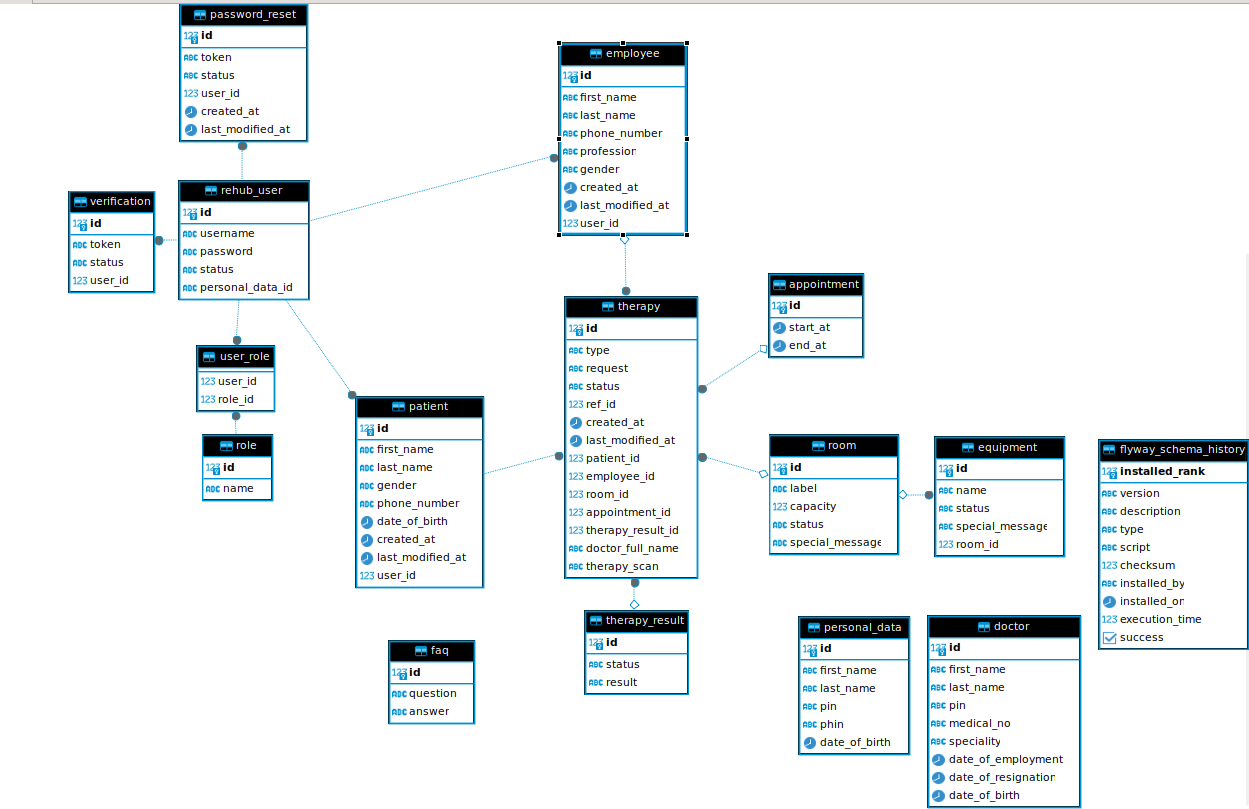
\includegraphics[scale=0.15]{dijagrami/rehub_db_diagram.png}
			         \centering
			         \caption{Dijagram baze podataka}
			         \label{fig:dbDiagram}
		        \end{figure}

			\eject

			
		\section{Dijagram razreda}
		
			Dijagramom razreda prikazujemo razrede u sustavu, njihove atribute i metode te veze između razreda koji se nasljeđuju ili međusobno komuniciraju. U nastavku slijede dijagrami čiji razredi imaju sličnu funkcionalnost i razinu apstrakcije.\\

            EntityClassDiagram - prikazuje razrede koji pripadaju sloju Model. Svaki od razreda se preslikava u odgovarajuću tablicu u bazi.\\

            RepositoryClassDiagram – prikazuje razrede koji pripadaju sloju Repository. Ovaj sloj komunicira sa bazom podataka i sa slojem Service.\\

            ServiceClassDiagram – prikazuje razrede koji pripadaju sloju Service. Ovaj sloj komunicira sa slojem Repository i Controller.\\

            ControllerClassDiagram – prikazuje razrede sloja Controller. Ovaj sloj komunicira sa slojem Service i s frontend dijelom aplikacije.\\

            EnumClassDiagram – prikazuje enumeracije koje koristi sloj Model.\\

            ConfigClassDiagram – prikazuje razrede sloja Config. Ovaj sloj služi za sigurnosne potrebe i komuniciranje putem e-maila.\\

            RequestClassDiagram – prikazuje razrede sloja Request. Ovaj sloj komunicira sa slojem Controller u svrhu validacije Post Request-a.\\

            ResponseClassDiagram – prikazuje razrede sloja Response. Ovaj sloj komunicira sa slojem Controller u svrhu vraćanja Response poruke.
			
			\begin{figure}[H]
			         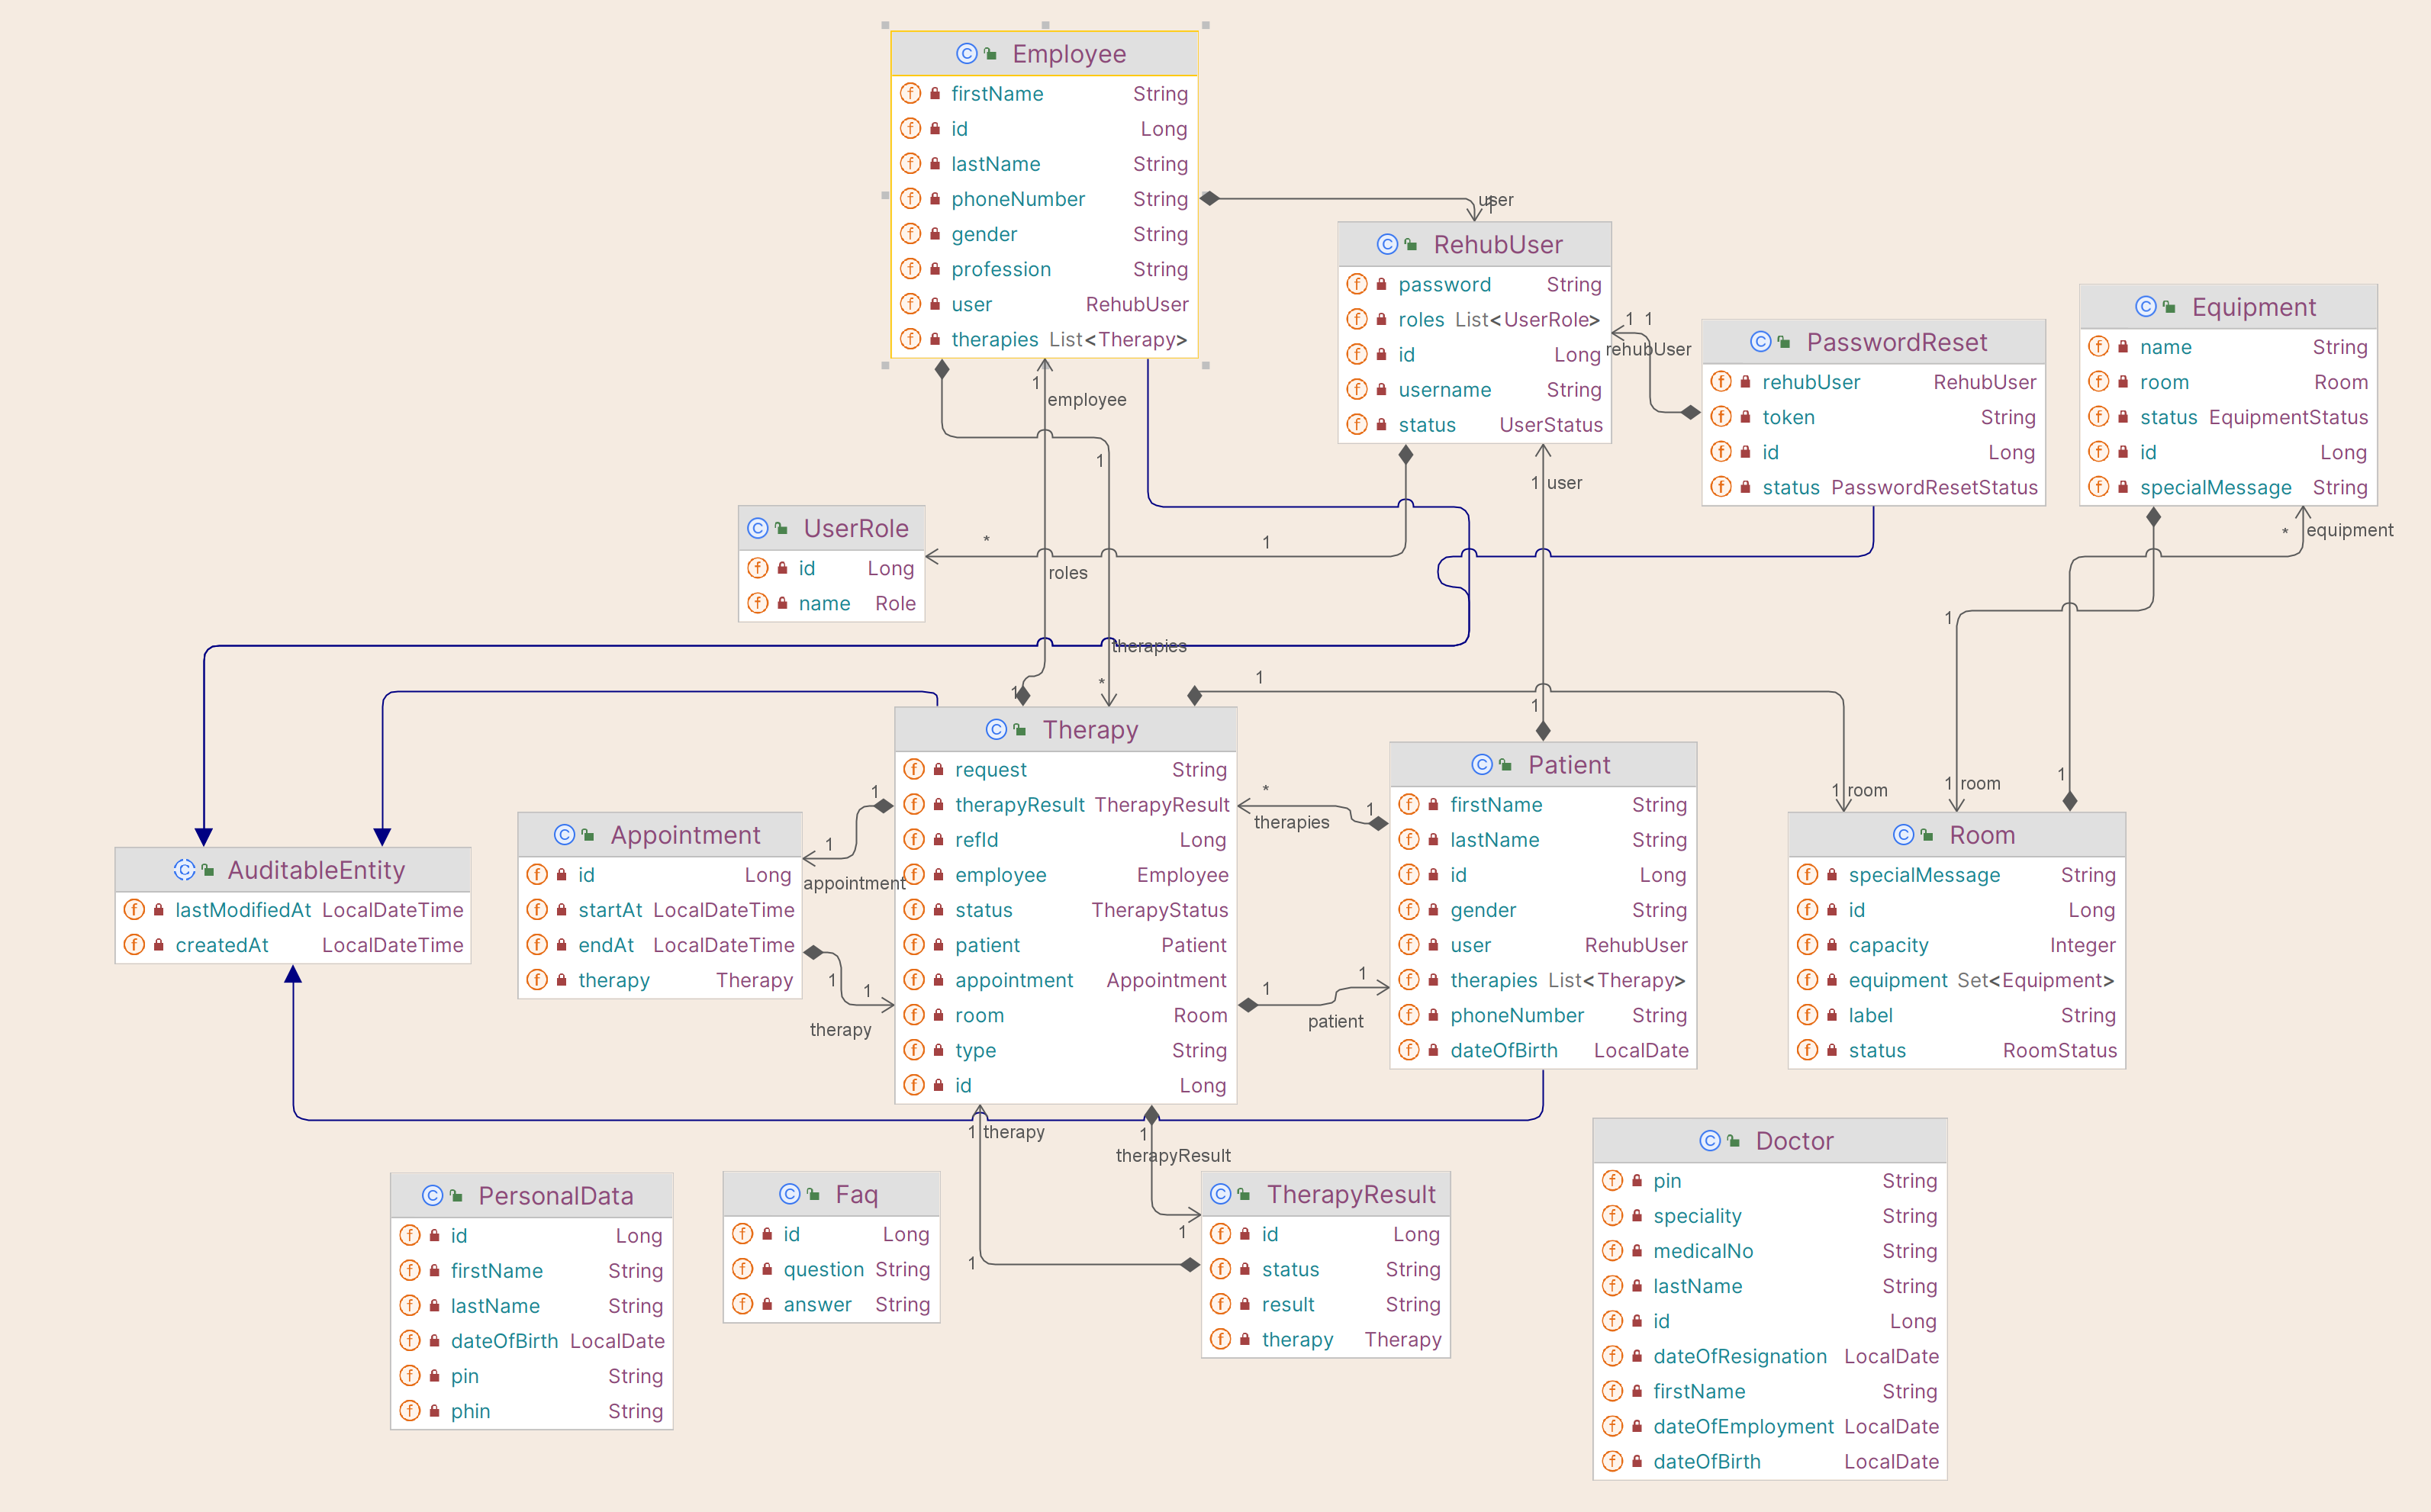
\includegraphics[scale=0.15]{dijagrami/EntityClassDiagram.png}
			         \centering
			         \caption{Dijagram razreda (Model)}
			         \label{fig:EntityClassDiagram}
		          \end{figure}

            \begin{figure}[H]
			         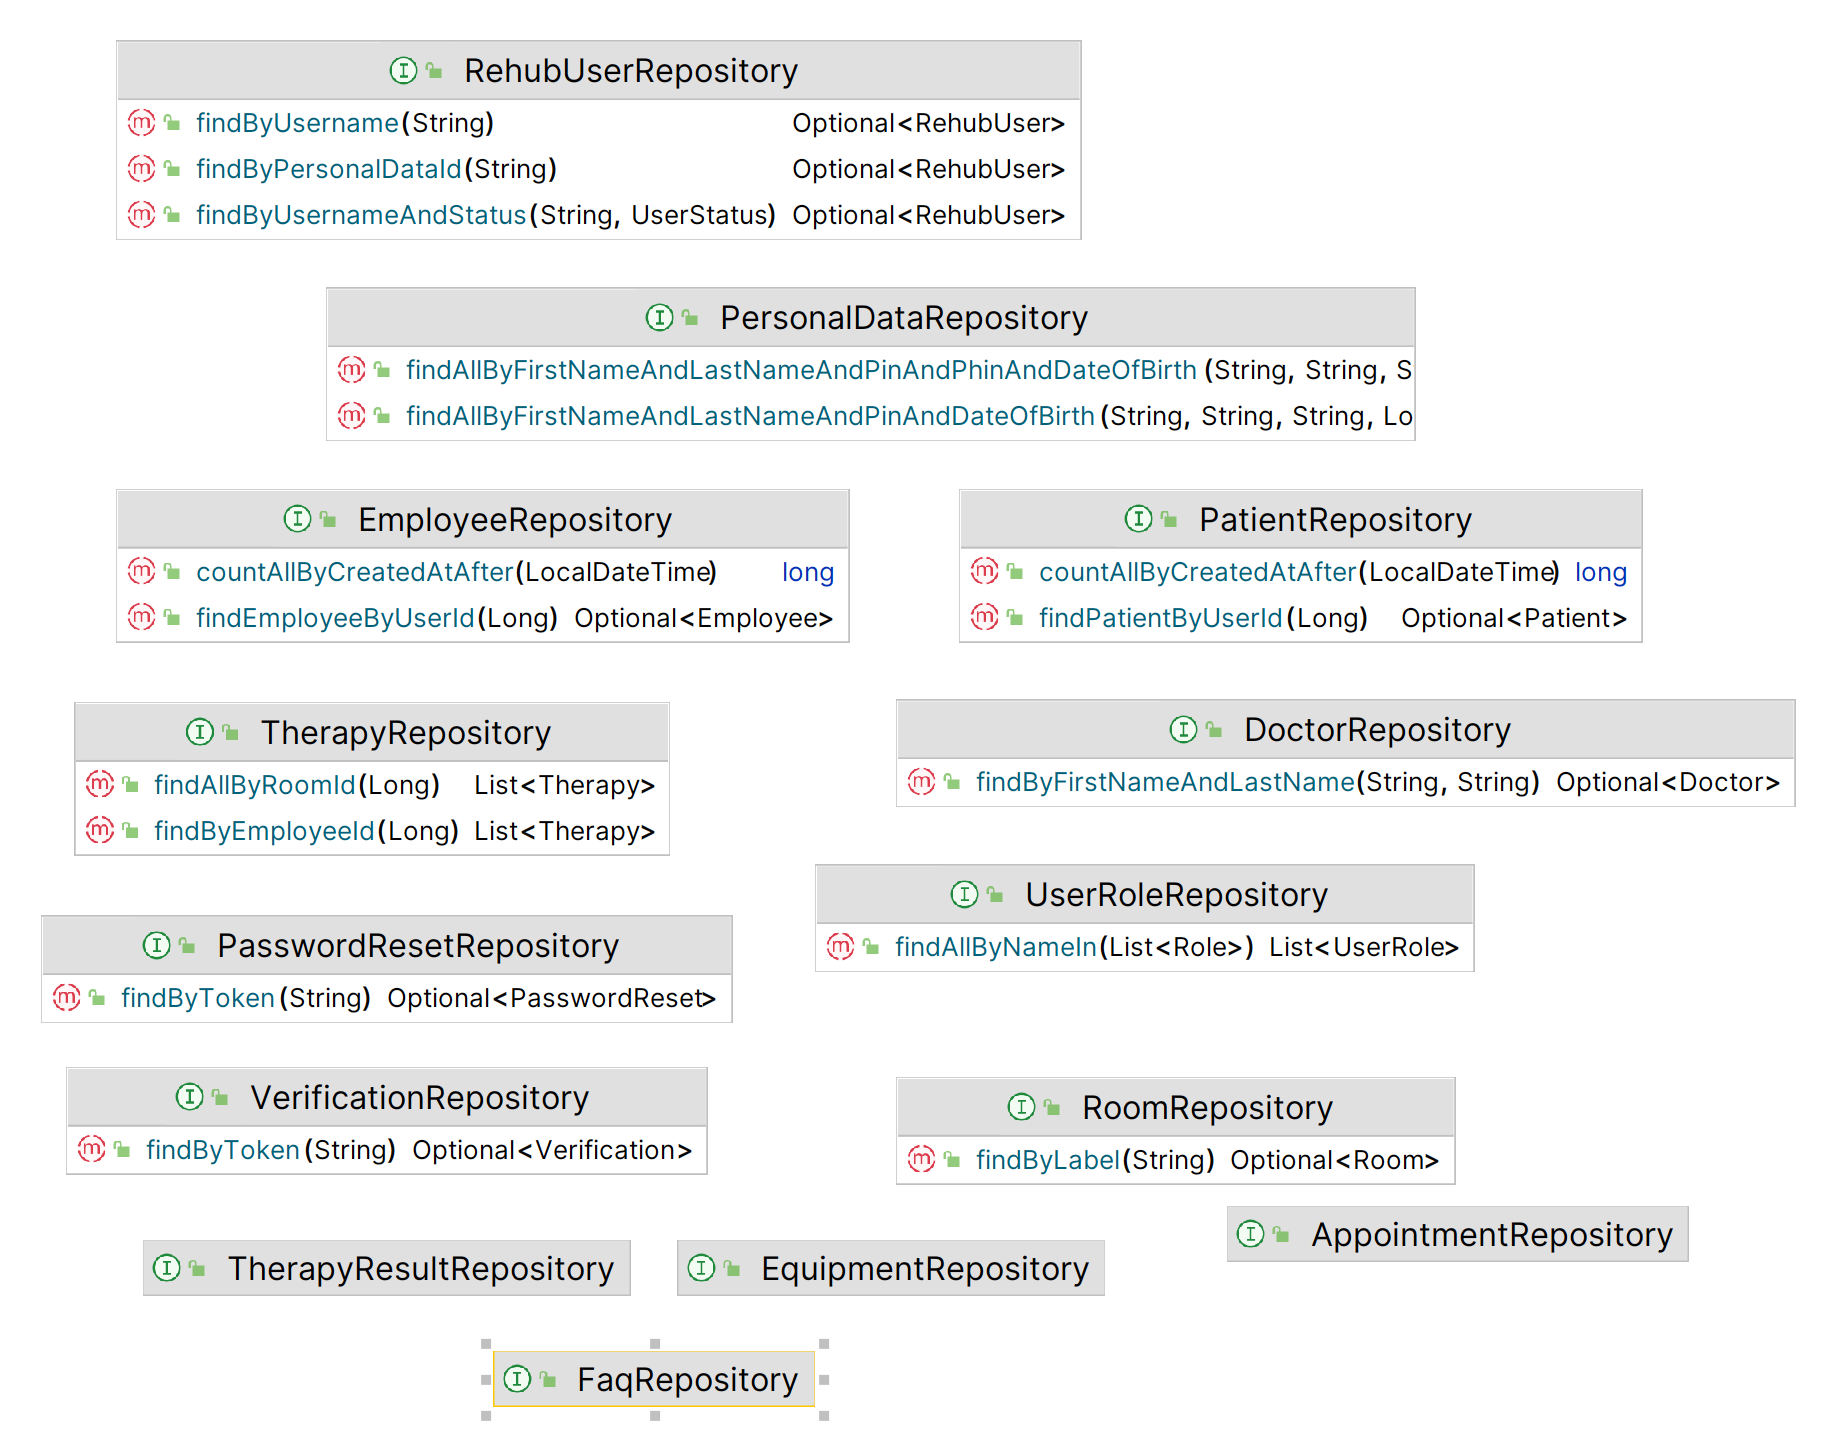
\includegraphics[scale=0.22]{dijagrami/RepositoryClassDiagram.png}
			         \centering
			         \caption{Dijagram razreda (Repository)}
			         \label{fig:RepositoryClassDiagram}
		          \end{figure}

            \begin{figure}[H]
			         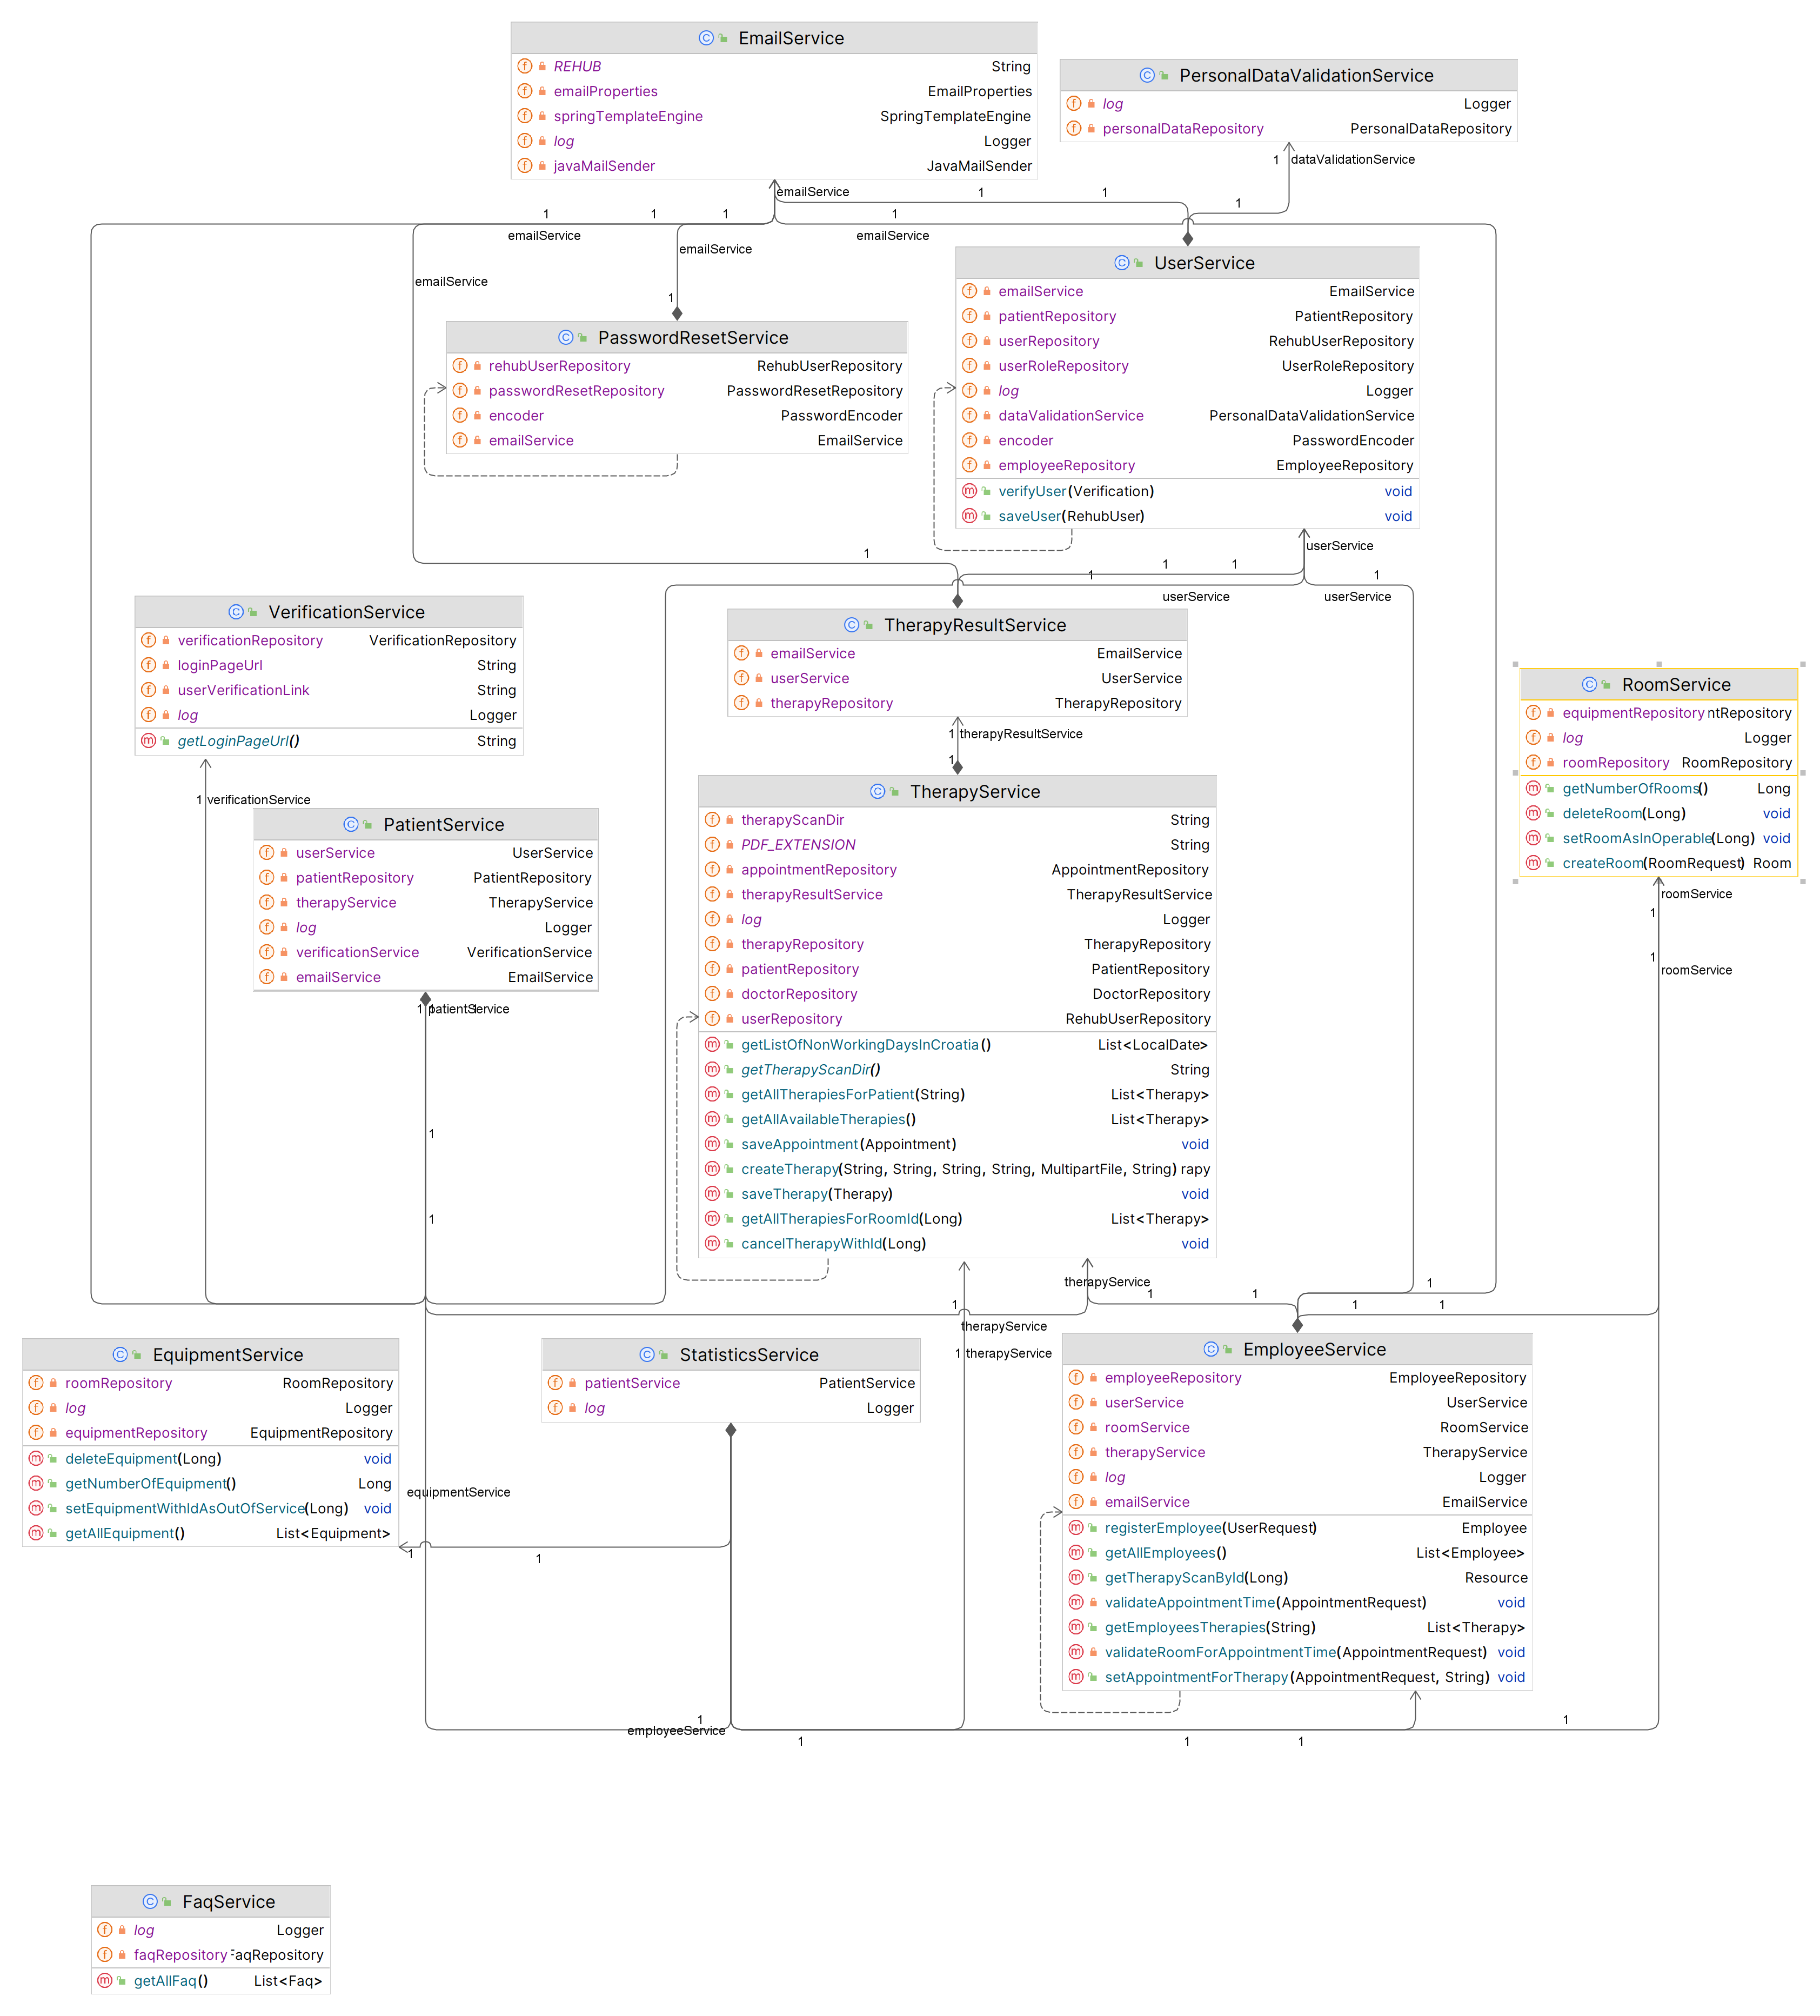
\includegraphics[scale=0.1]{dijagrami/ServiceClassDiagram.png}
			         \centering
			         \caption{Dijagram razreda (Service)}
			         \label{fig:ServiceClassDiagram}
		          \end{figure}

            \begin{figure}[H]
			         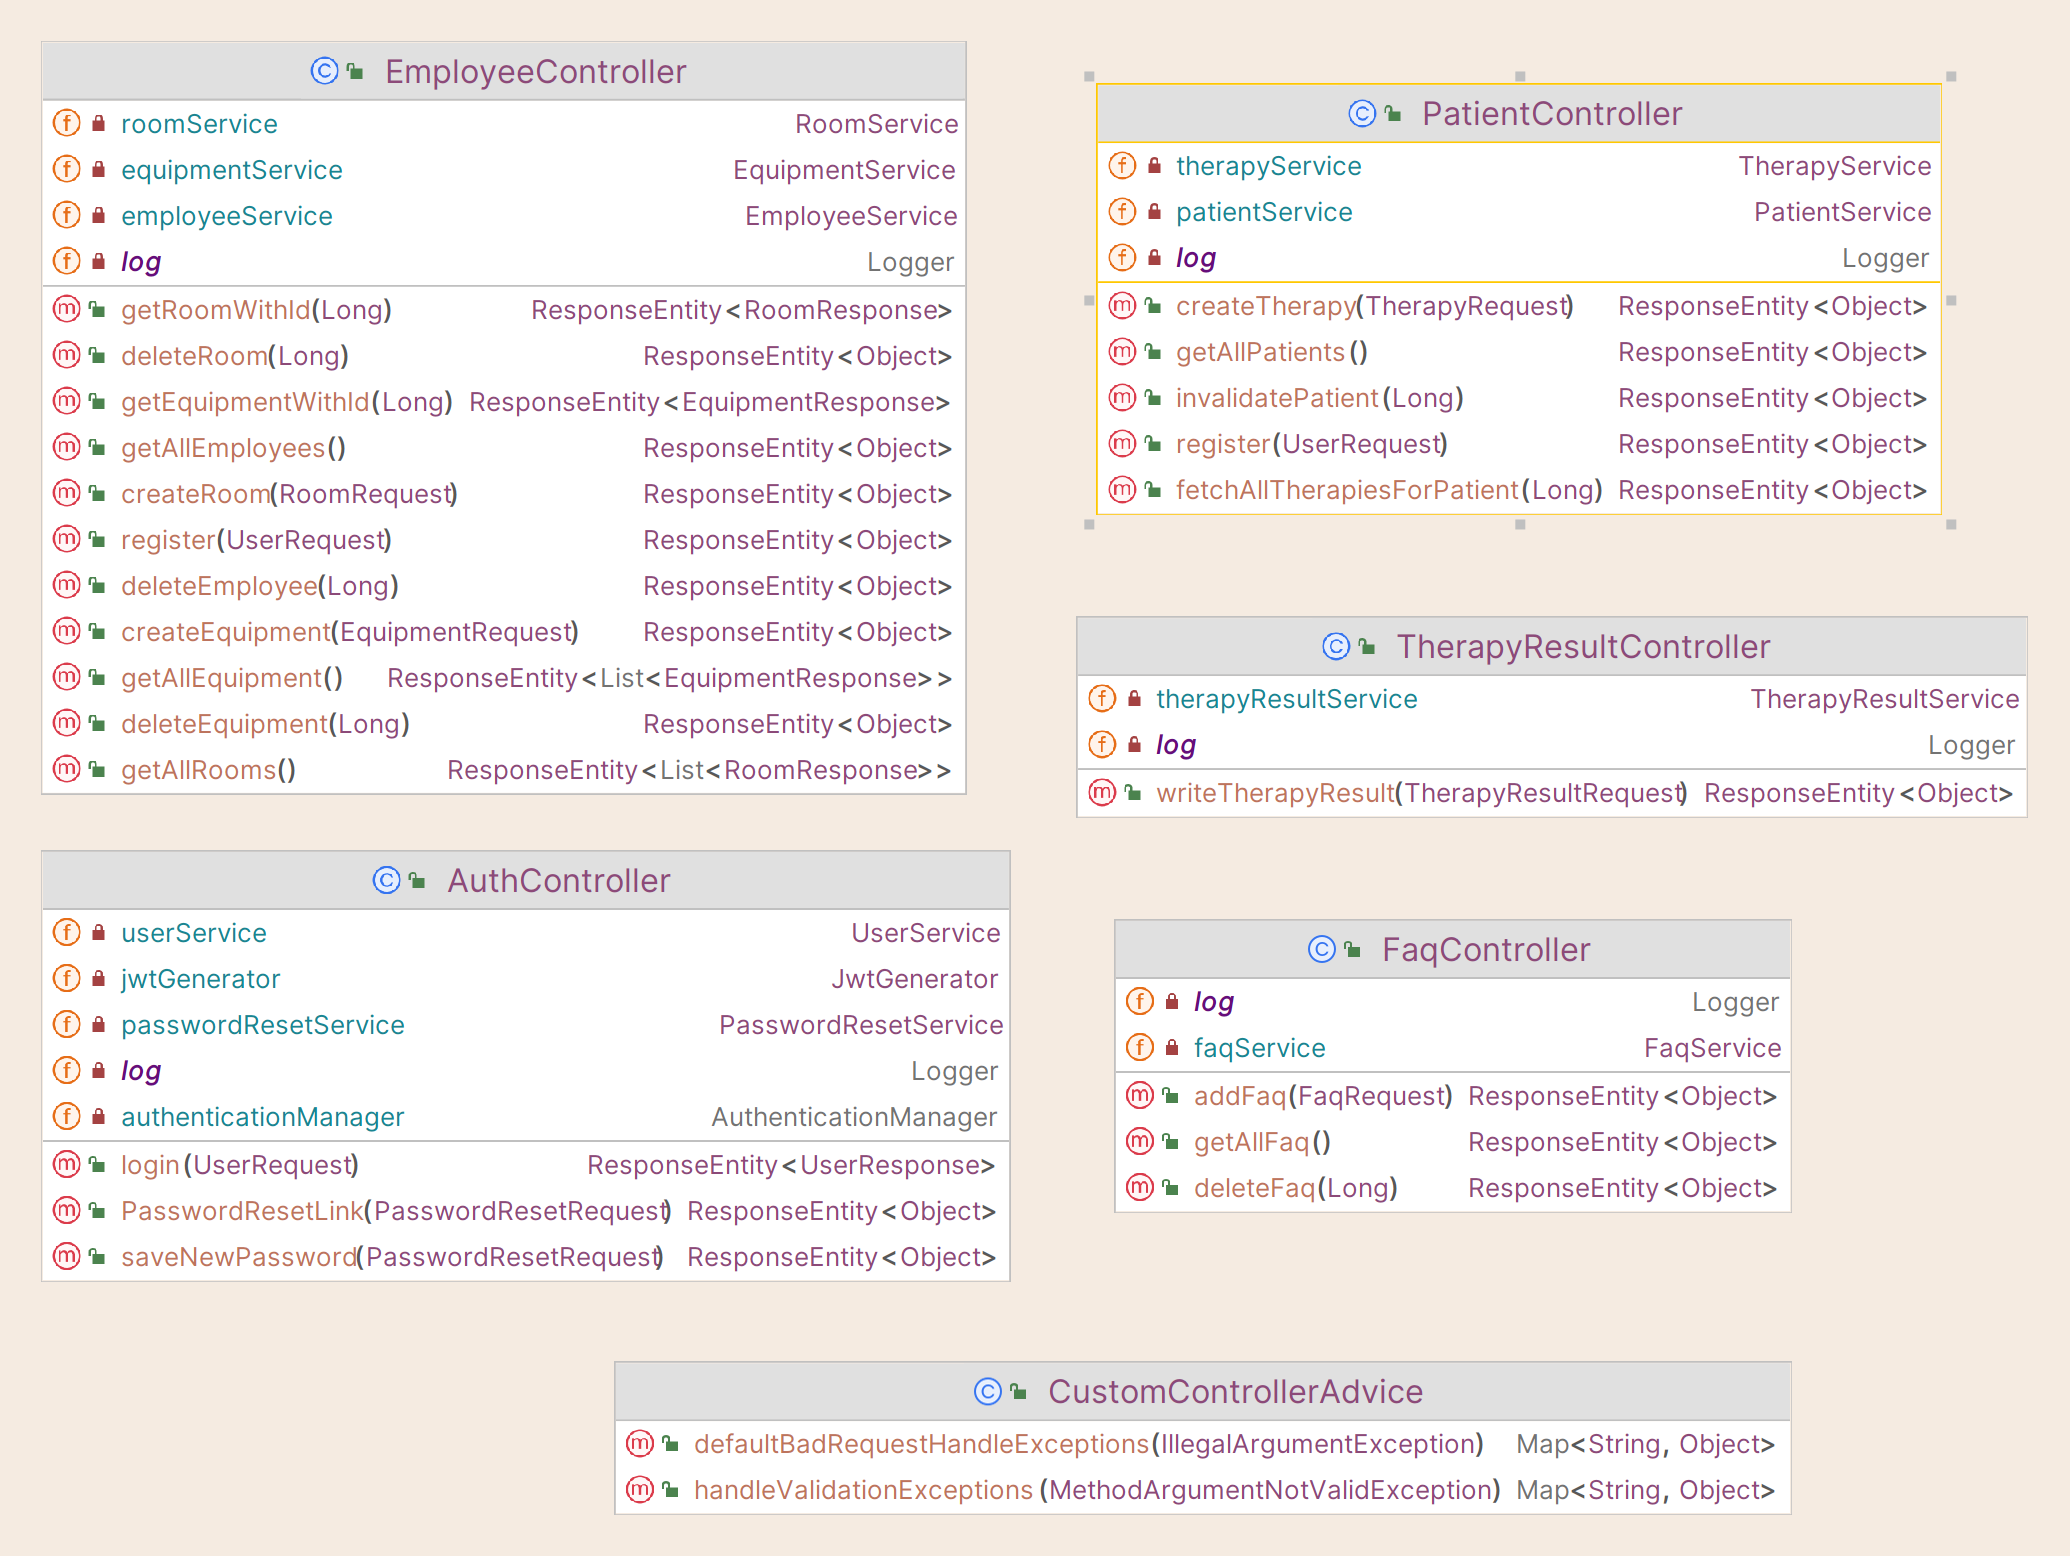
\includegraphics[scale=0.2]{dijagrami/ControllerClassDiagram.png}
			         \centering
			         \caption{Dijagram razreda (Controller)}
			         \label{fig:ControllerClassDiagram}
		          \end{figure}

            \begin{figure}[H]
			         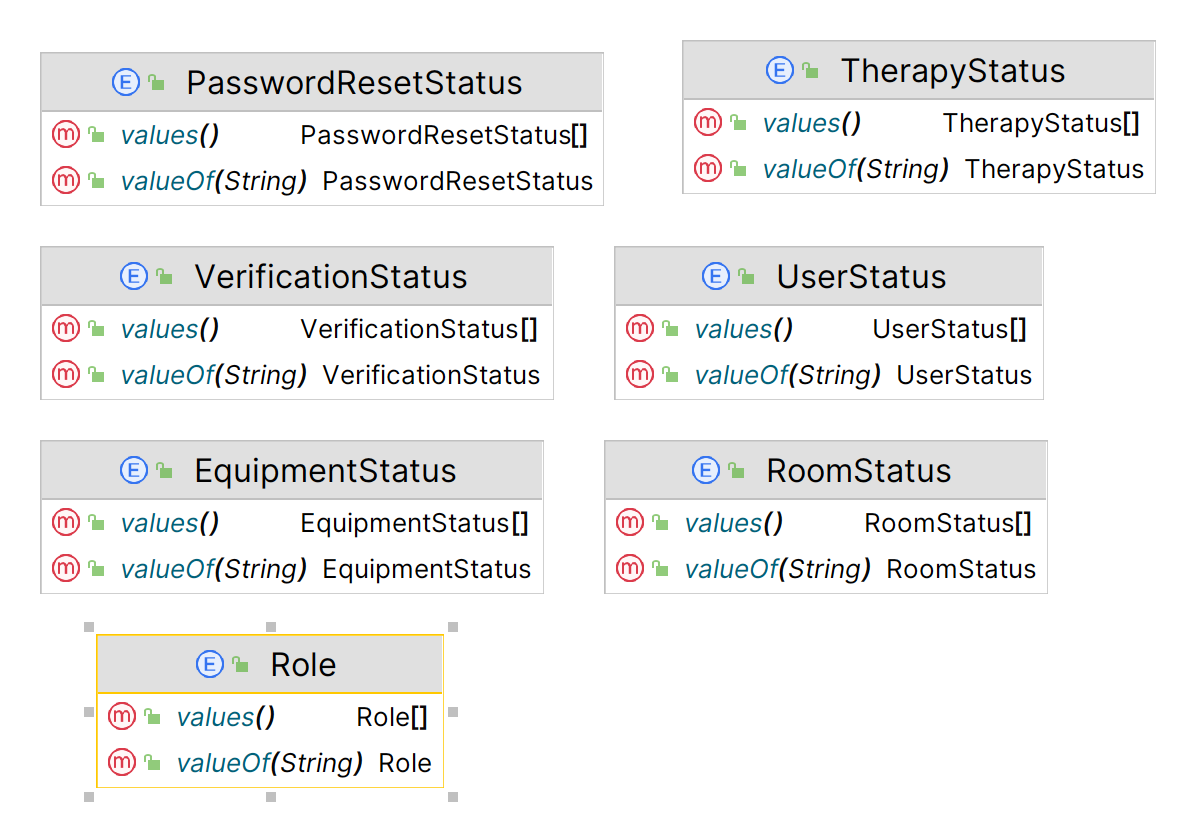
\includegraphics[scale=0.2]{dijagrami/EnumClassDiagram.png}
			         \centering
			         \caption{Dijagram enumeracija (Model)}
			         \label{fig:EnumClassDiagram}
		          \end{figure}

            \begin{figure}[H]
			         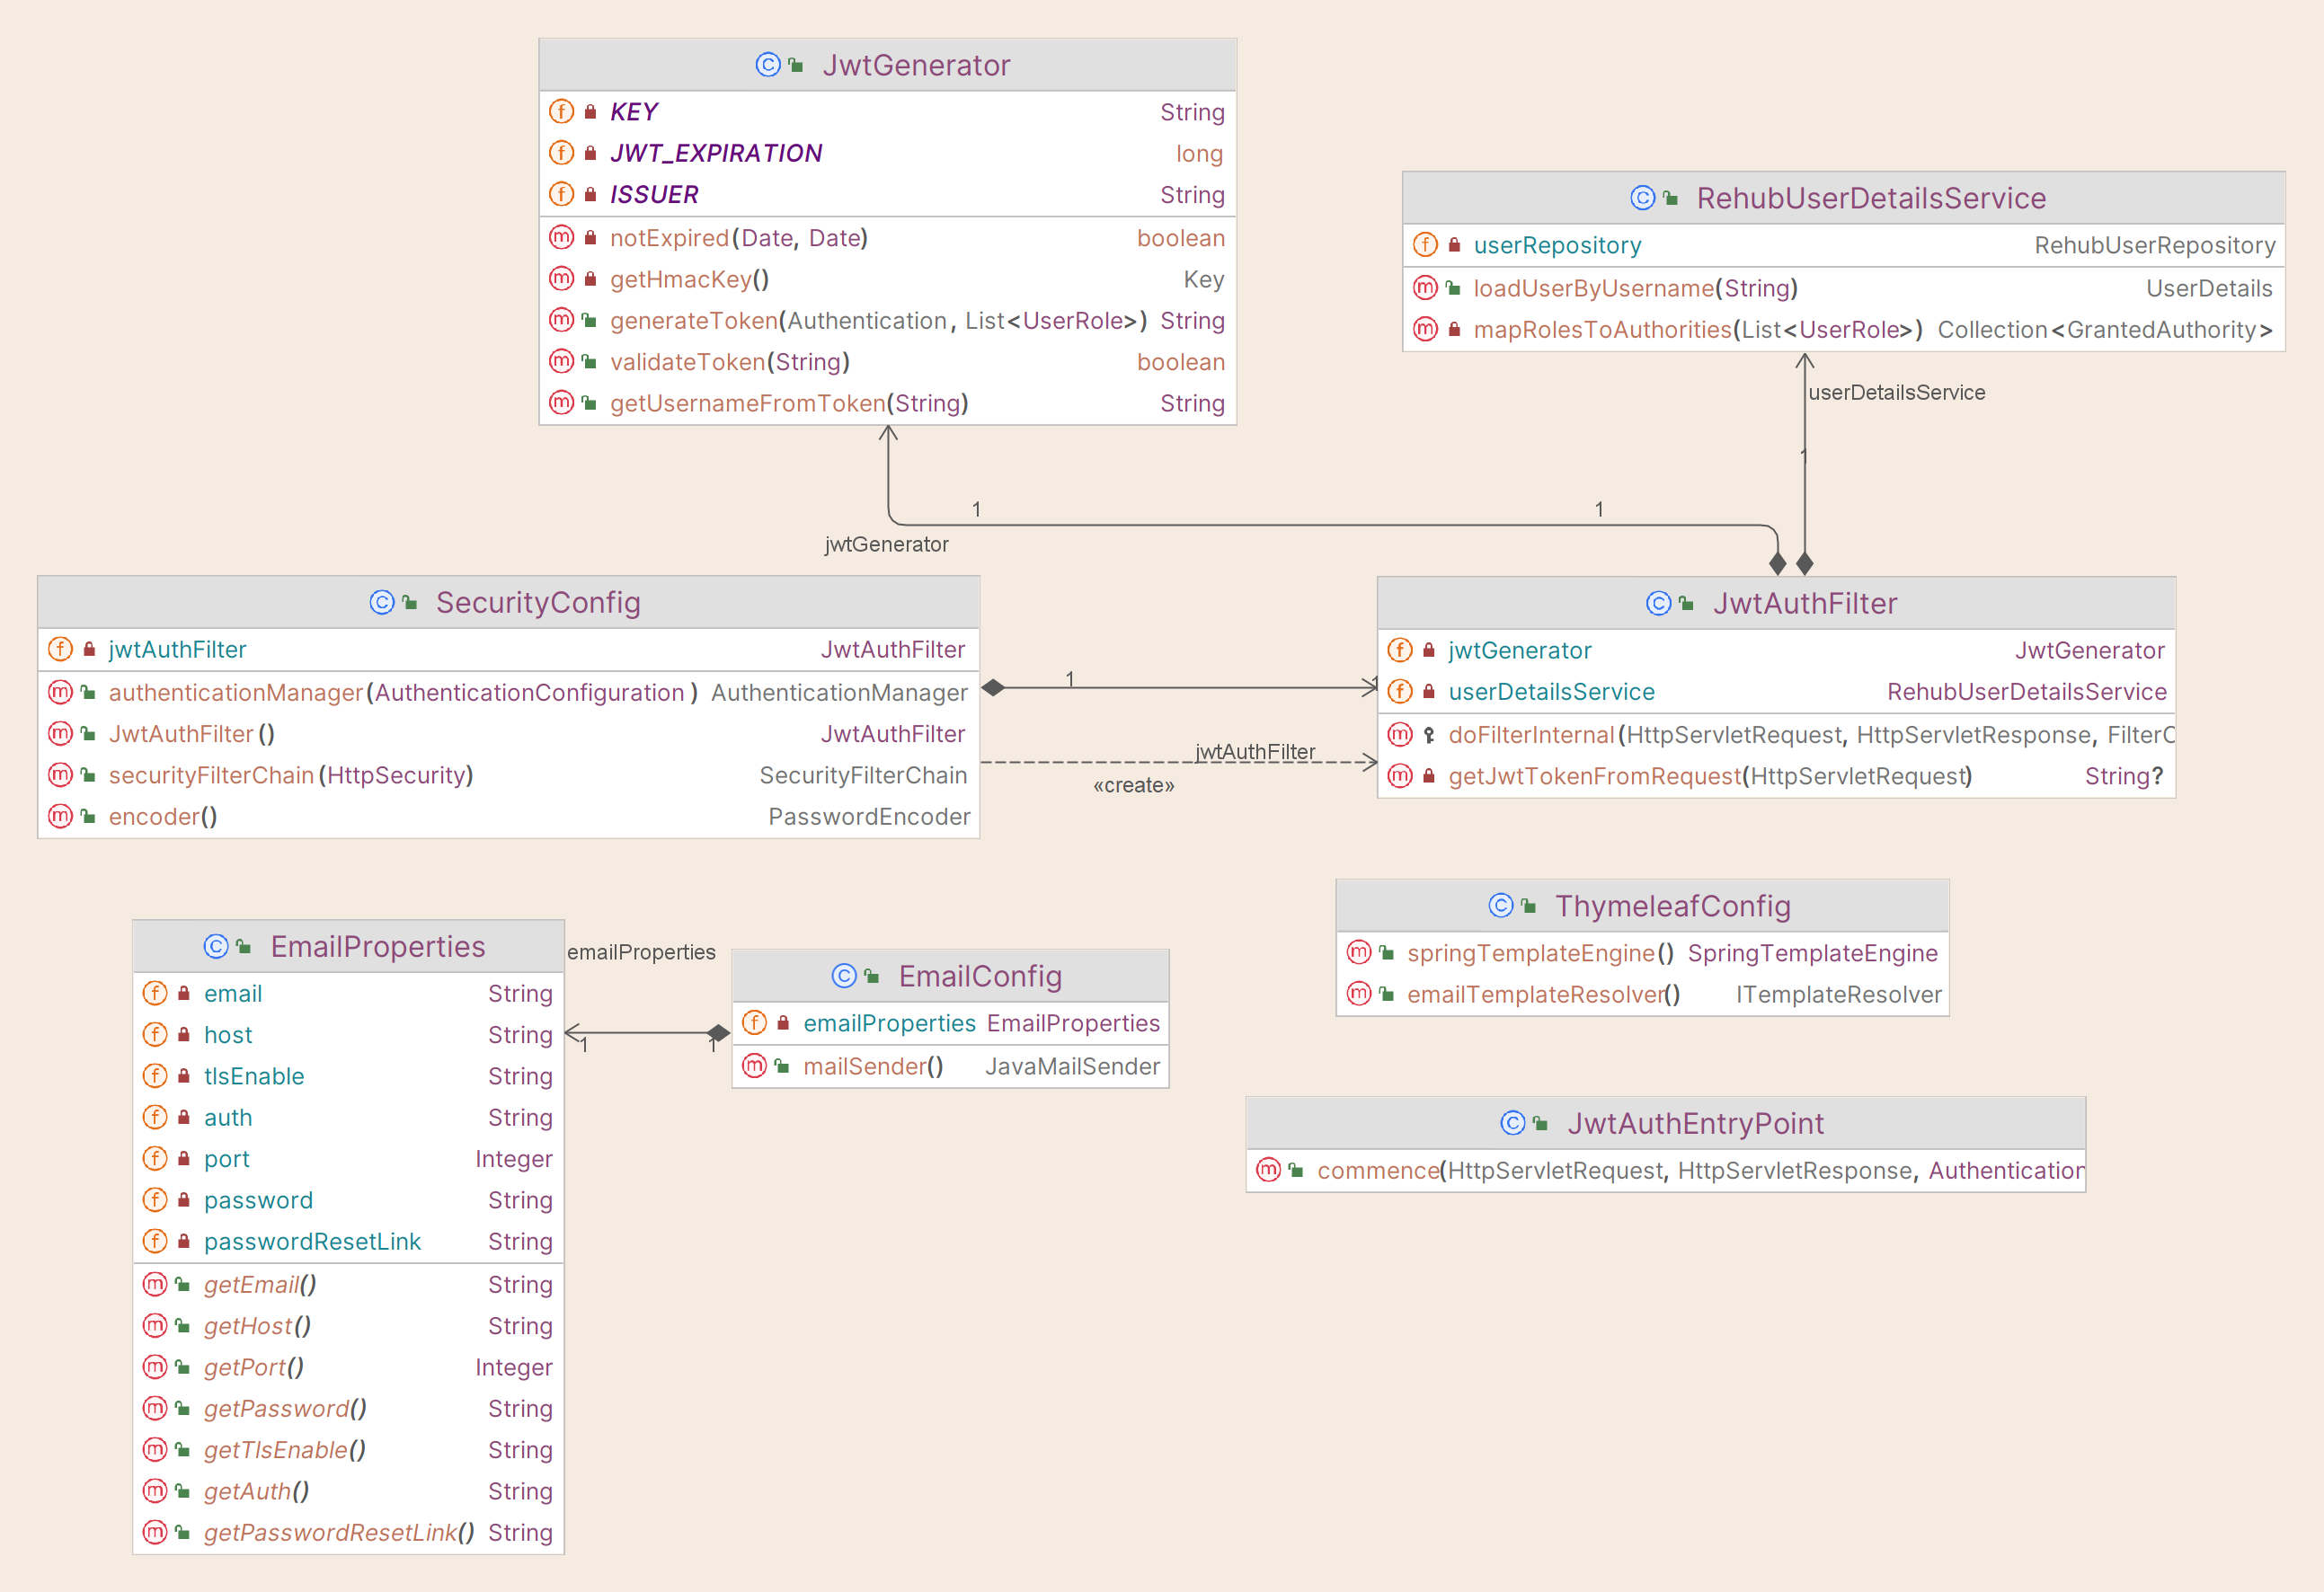
\includegraphics[scale=0.18]{dijagrami/ConfigClassDiagram.png}
			         \centering
			         \caption{Dijagram razreda (Config)}
			         \label{fig:ConfigClassDiagram}
		          \end{figure}

            \begin{figure}[H]
			         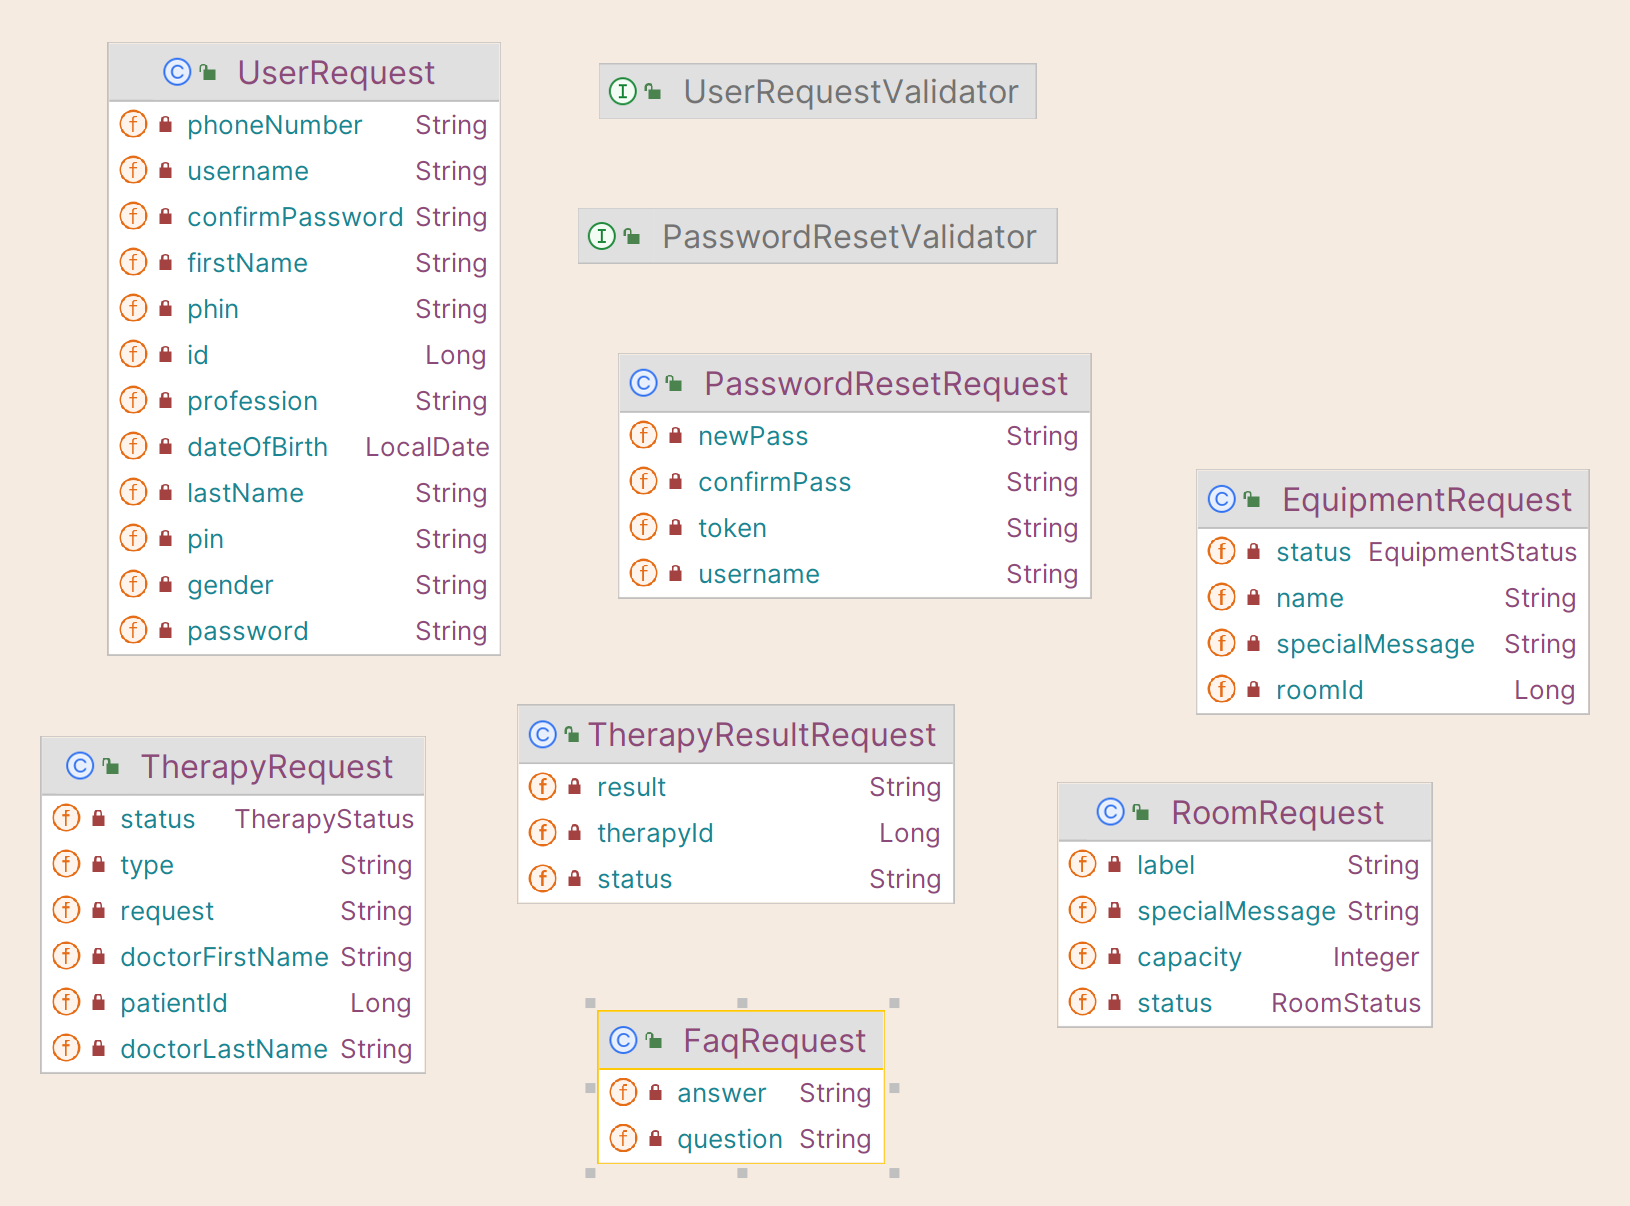
\includegraphics[scale=0.18]{dijagrami/RequestClassDiagrams.png}
			         \centering
			         \caption{Dijagram razreda (Request)}
			         \label{fig:RequestClassDiagrams}
		          \end{figure}

            \begin{figure}[H]
			         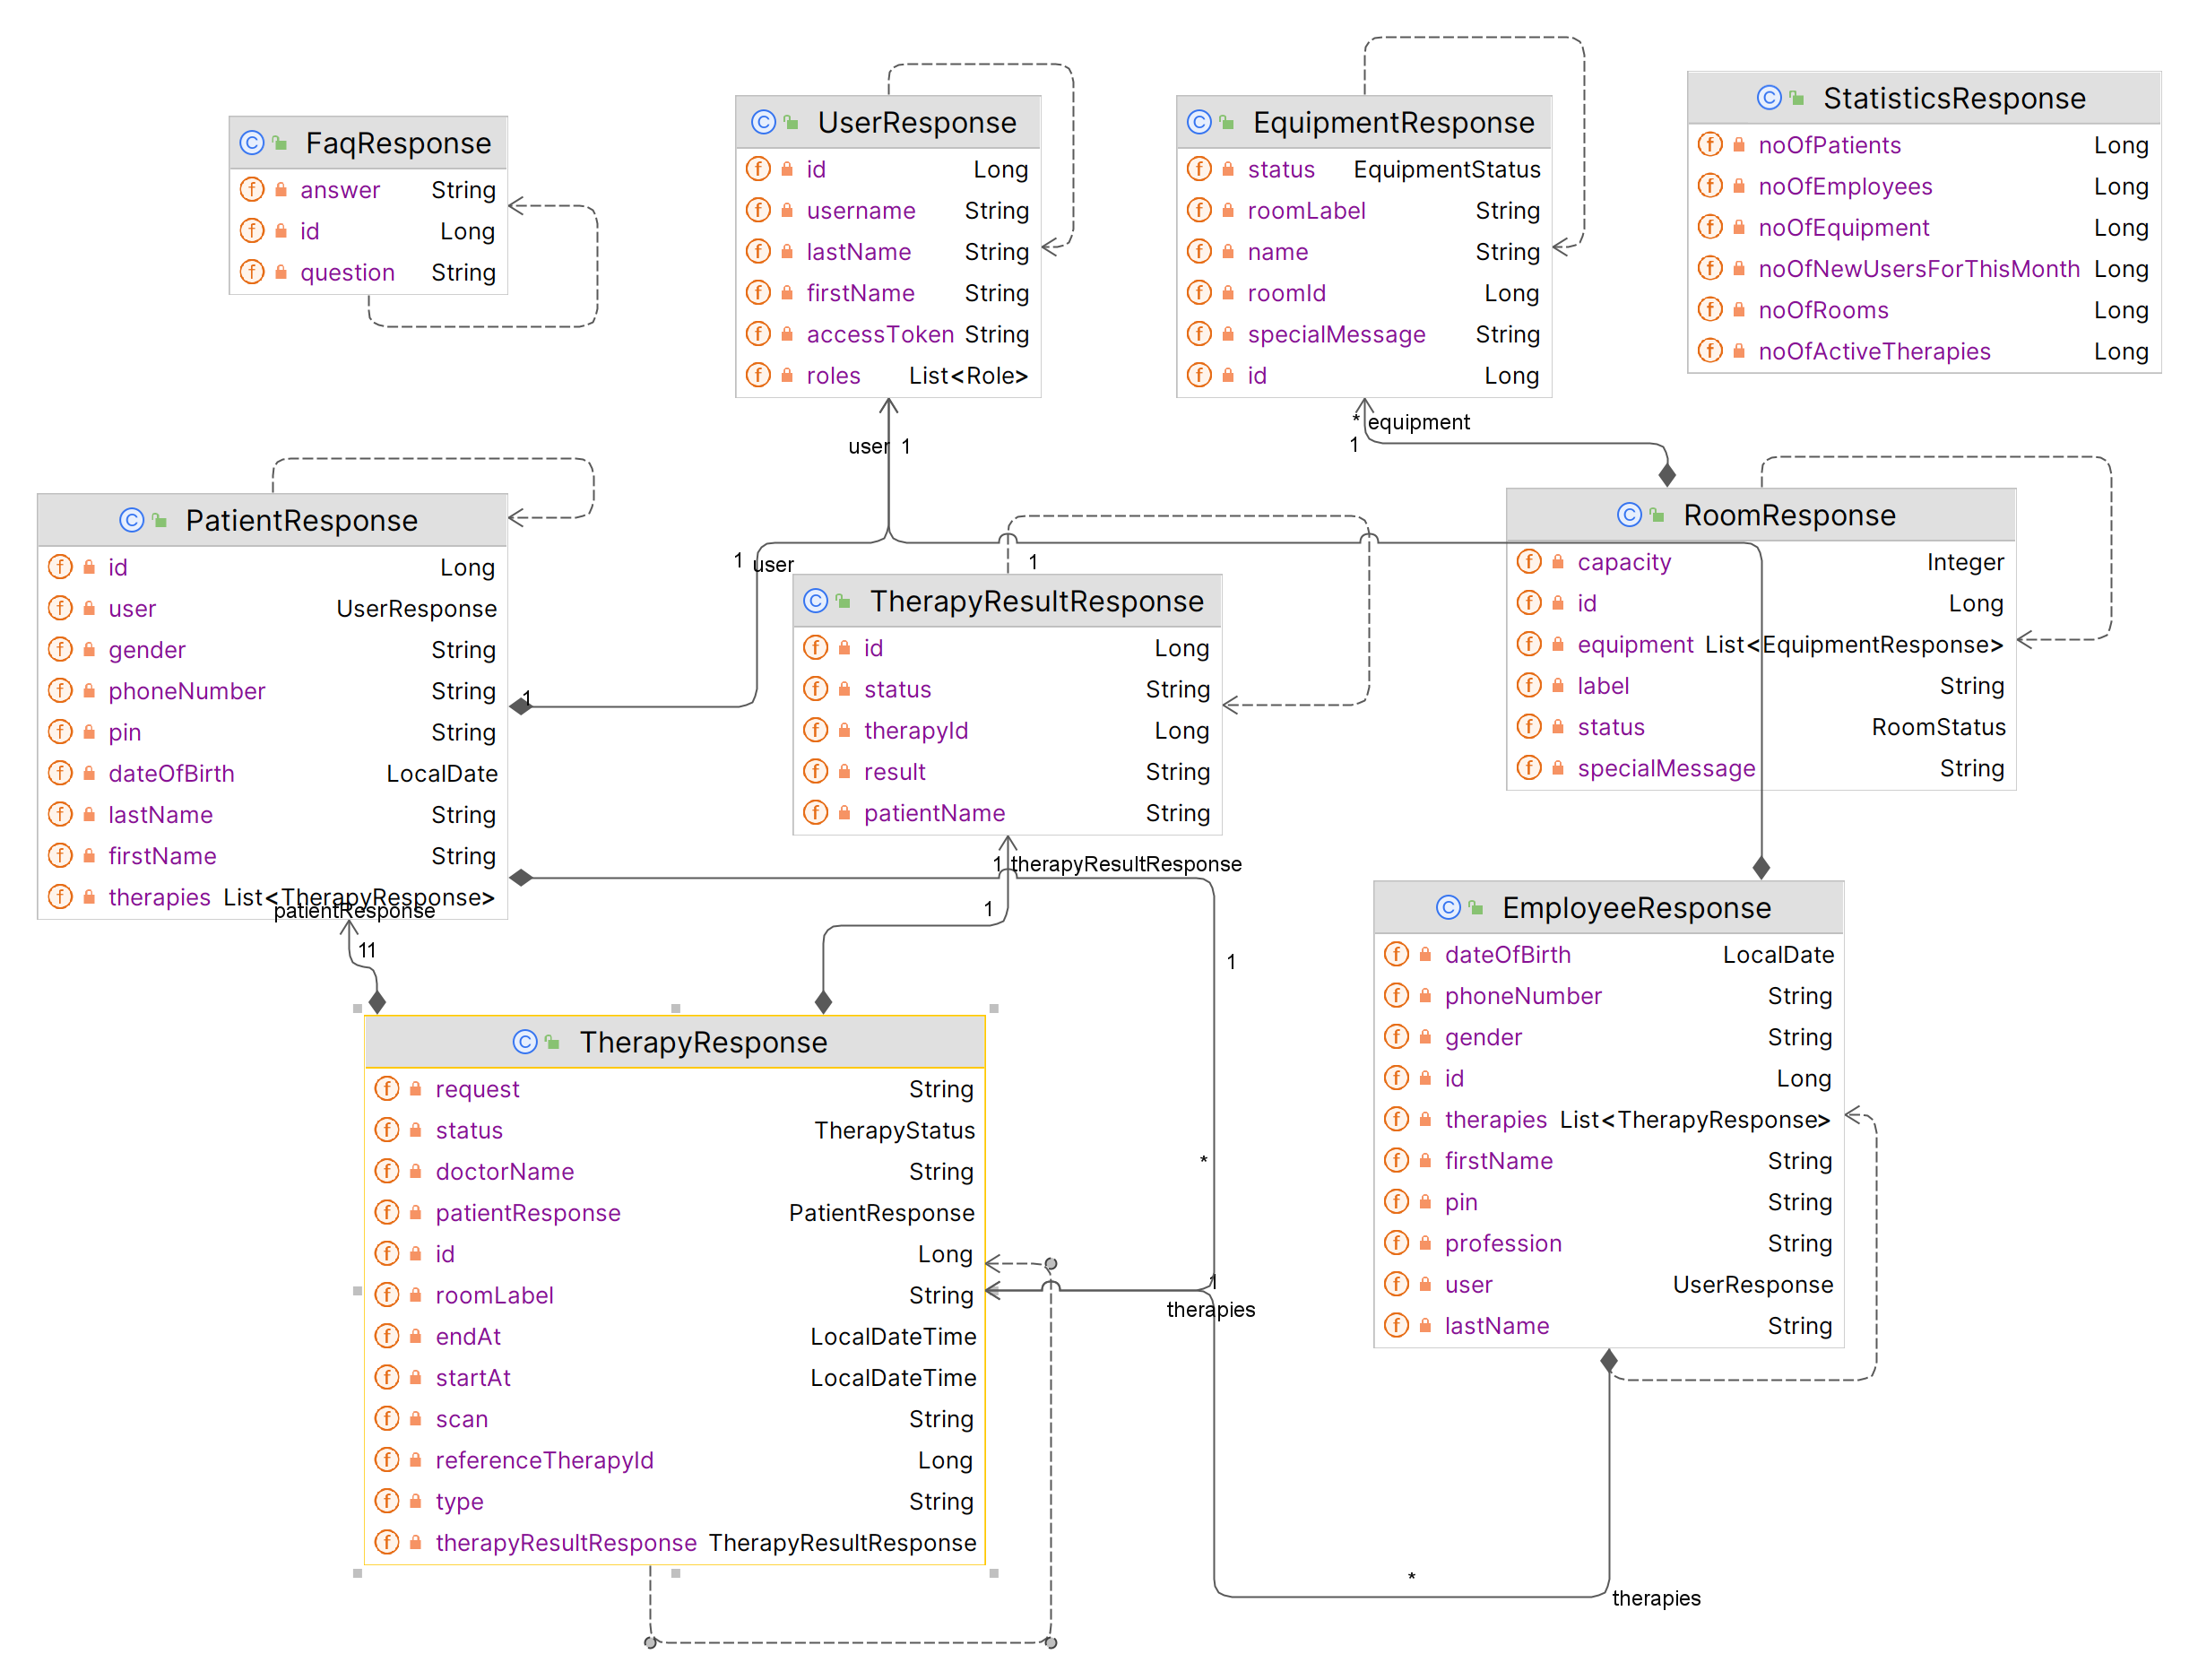
\includegraphics[scale=0.13]{dijagrami/ResponseClassDiagram.png}
			         \centering
			         \caption{Dijagram razreda (Response)}
			         \label{fig:ResponseClassDiagram}
		          \end{figure}
			
			
			
			\eject
		
		\section{Dijagram stanja}
			
			
			

            
			
			\eject 
		
		\section{Dijagram aktivnosti}
			
			\textbf{\textit{dio 2. revizije}}\\
			
			 \textit{Potrebno je priložiti dijagram aktivnosti s pripadajućim opisom. Dijagram aktivnosti treba prikazivati značajan dio sustava.}
			
			\eject
		\section{Dijagram komponenti}

            Dijagram komponenti detaljno opisuje strukturu sustava, međusobne veze između komponenti te njihove odnose s okolinom. Prikazuje integraciju frontend i backend aplikacija putem REST API-ja. Backend aplikacija je složena od servisa, repozitorija i kontrolera. Repozitorij komunicira s bazom podataka putem SQL upita kako bi dohvatio potrebne podatke. Servis komunicira s repozitorijem i kontrolerom. Kontroler obrađuje dolazne zahtjeve s frontenda. Frontend aplikacija obuhvaća routere, komponente, servise te razne biblioteke. Router je komponenta koja, na temelju korisničkog zahtjeva za određeni URL, određuje koja datoteka (stranica) će biti isporučena. Komponente predstavljaju stranice koje se isporučuju kao JavaScript datoteke (HTML, CSS, JavaScript kod) ovisne o React biblioteci. Servisi imaju ulogu zahtjeva prema backendu, validacije i sličnih zadataka. Axios, kao biblioteka HTTP klijenta, pojednostavljuje slanje HTTP zahtjeva prema REST API-ju, odnosno prema backend aplikaciji.
    
			    \begin{figure}[H]
			         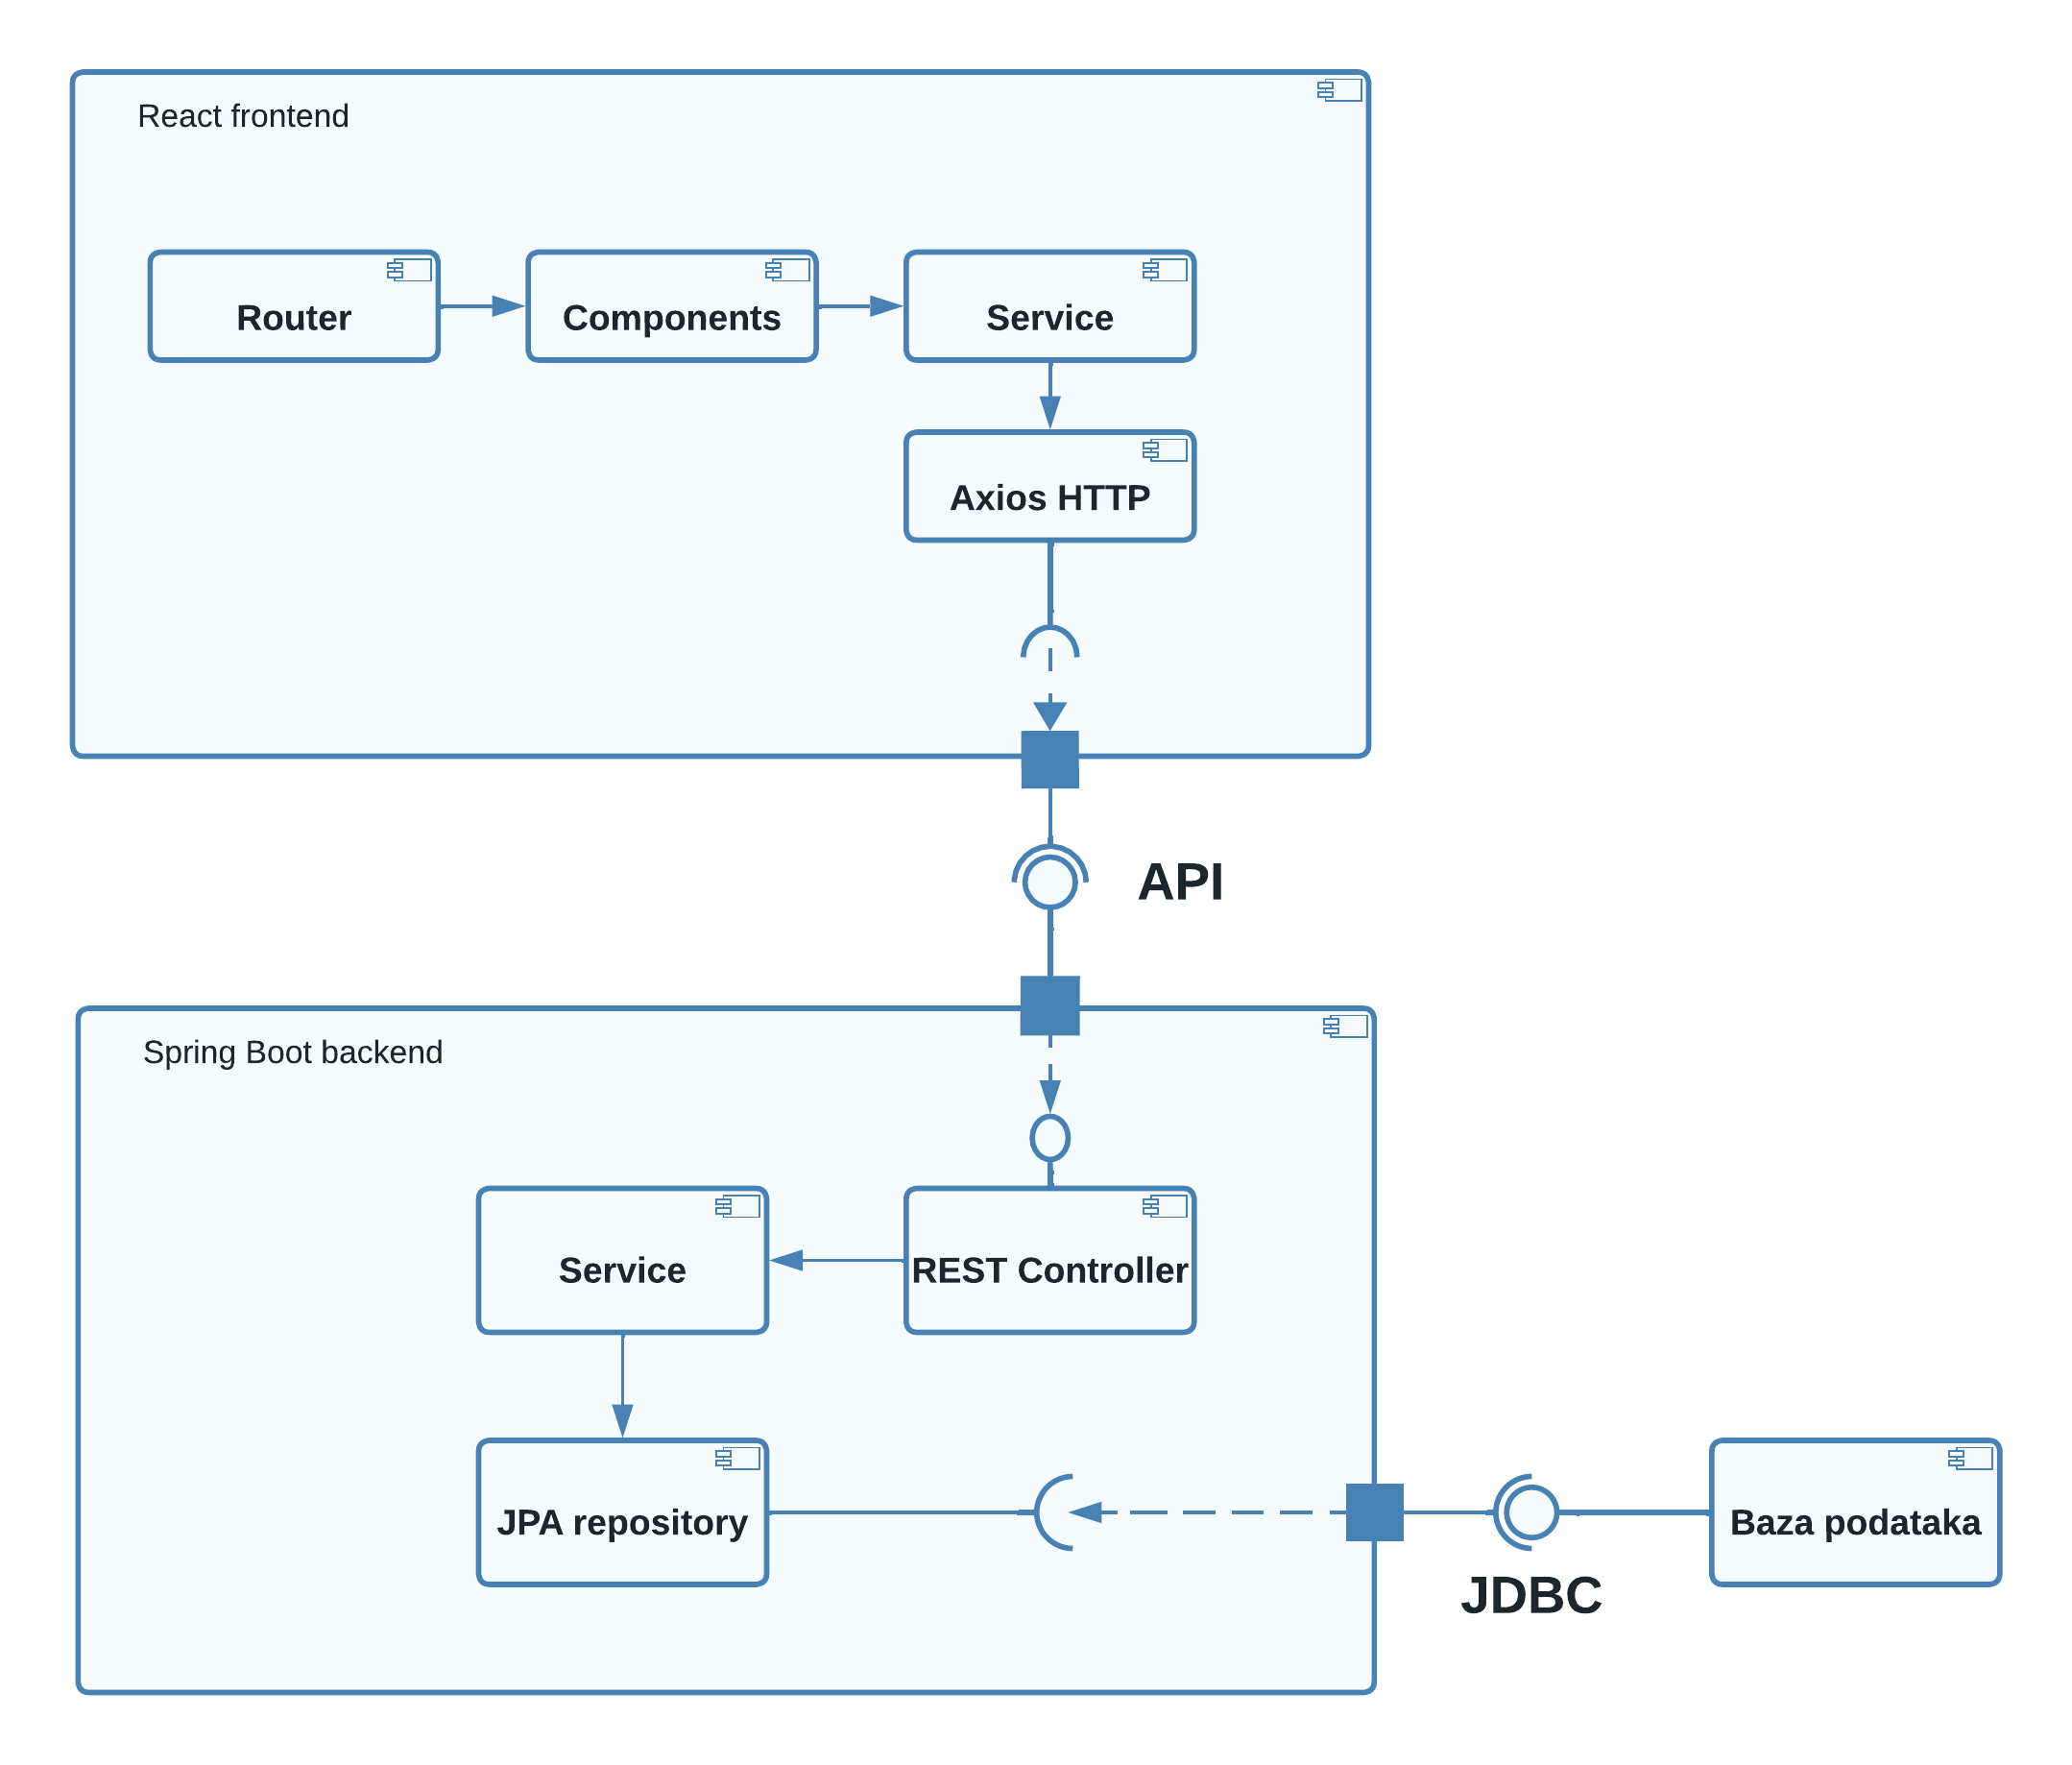
\includegraphics[scale=0.17]{dijagrami/component_diagram.png}
			         \centering
			         \caption{Dijagram komponenti}
			         \label{fig:component_diagram}
		        \end{figure}